\documentclass[USenglish,cleveref, autoref, thm-restate]{lipics-v2019}
\usepackage{listings,hyperref,multirow,paralist,xspace,url,wrapfig}
\newcommand{\missingTag}[1]{\textcolor{red}{#1}\xspace}
\newcommand{\missingNumber}{\textcolor{red}{XX}\xspace}
\newcommand{\missingPercentage}{\textcolor{red}{XX\%}\xspace}
\newcommand{\missingTable}[1][XX]{\textcolor{red}{Table #1}\xspace}
\newcommand{\missingGraph}{\textcolor{red}{XXGraph}\xspace}


%\newcommand{\CoreEvalCallCountRnd}{12.6M\xspace}
\newcommand{\CoreEvalCallCount}{12,637,139\xspace}
\newcommand{\CoreEvalSiteCountRnd}{170\xspace}
\newcommand{\CoreEvalSiteCount}{170\xspace}
\newcommand{\CoreEvalParentCallCountRnd}{254.1K\xspace}
\newcommand{\CoreEvalParentCallCount}{254,112\xspace}
\newcommand{\CoreEvalParentSiteCountRnd}{16\xspace}
\newcommand{\CoreEvalParentSiteCount}{16\xspace}
\newcommand{\CoreEvalqCallCountRnd}{265.5K\xspace}
\newcommand{\CoreEvalqCallCount}{265,499\xspace}
\newcommand{\CoreEvalqSiteCountRnd}{4\xspace}
\newcommand{\CoreEvalqSiteCount}{4\xspace}
\newcommand{\CoreLocalCallCountRnd}{234.2K\xspace}
\newcommand{\CoreLocalCallCount}{234,212\xspace}
\newcommand{\CoreLocalSiteCountRnd}{1.1K\xspace}
\newcommand{\CoreLocalSiteCount}{1,116\xspace}
\newcommand{\PackageEvalCallCountRnd}{5M\xspace}
\newcommand{\PackageEvalCallCount}{5,021,240\xspace}
\newcommand{\PackageEvalSiteCountRnd}{2.4K\xspace}
\newcommand{\PackageEvalSiteCount}{2,448\xspace}
\newcommand{\PackageEvalParentCallCountRnd}{52.1K\xspace}
\newcommand{\PackageEvalParentCallCount}{52,130\xspace}
\newcommand{\PackageEvalParentSiteCountRnd}{351\xspace}
\newcommand{\PackageEvalParentSiteCount}{351\xspace}
\newcommand{\PackageEvalqCallCountRnd}{292\xspace}
\newcommand{\PackageEvalqCallCount}{292\xspace}
\newcommand{\PackageEvalqSiteCountRnd}{7\xspace}
\newcommand{\PackageEvalqSiteCount}{7\xspace}
\newcommand{\PackageLocalCallCountRnd}{1.3K\xspace}
\newcommand{\PackageLocalCallCount}{1,251\xspace}
\newcommand{\PackageLocalSiteCountRnd}{8\xspace}
\newcommand{\PackageLocalSiteCount}{8\xspace}
\newcommand{\KaggleEvalCallCountRnd}{0\xspace}
\newcommand{\KaggleEvalCallCount}{0\xspace}
\newcommand{\KaggleEvalSiteCountRnd}{0\xspace}
\newcommand{\KaggleEvalSiteCount}{0\xspace}
\newcommand{\KaggleEvalParentCallCountRnd}{0\xspace}
\newcommand{\KaggleEvalParentCallCount}{0\xspace}
\newcommand{\KaggleEvalParentSiteCountRnd}{0\xspace}
\newcommand{\KaggleEvalParentSiteCount}{0\xspace}
\newcommand{\KaggleEvalqCallCountRnd}{0\xspace}
\newcommand{\KaggleEvalqCallCount}{0\xspace}
\newcommand{\KaggleEvalqSiteCountRnd}{0\xspace}
\newcommand{\KaggleEvalqSiteCount}{0\xspace}
\newcommand{\KaggleLocalCallCountRnd}{0\xspace}
\newcommand{\KaggleLocalCallCount}{0\xspace}
\newcommand{\KaggleLocalSiteCountRnd}{0\xspace}
\newcommand{\KaggleLocalSiteCount}{0\xspace}
\newcommand{\CoreAllCallCountRnd}{13.4M\xspace}
\newcommand{\CoreAllCallCount}{13,390,962\xspace}
\newcommand{\CoreAllSiteCountRnd}{1.3K\xspace}
\newcommand{\CoreAllSiteCount}{1,306\xspace}
\newcommand{\KaggleAllCallCountRnd}{0\xspace}
\newcommand{\KaggleAllCallCount}{0\xspace}
\newcommand{\KaggleAllSiteCountRnd}{0\xspace}
\newcommand{\KaggleAllSiteCount}{0\xspace}
\newcommand{\PackageAllCallCountRnd}{5.1M\xspace}
\newcommand{\PackageAllCallCount}{5,074,913\xspace}
\newcommand{\PackageAllSiteCountRnd}{2.8K\xspace}
\newcommand{\PackageAllSiteCount}{2,814\xspace}
\newcommand{\AllEvalCallCountRnd}{17.7M\xspace}
\newcommand{\AllEvalCallCount}{17,658,379\xspace}
\newcommand{\AllEvalSiteCountRnd}{2.6K\xspace}
\newcommand{\AllEvalSiteCount}{2,618\xspace}
\newcommand{\AllEvalParentCallCountRnd}{306.2K\xspace}
\newcommand{\AllEvalParentCallCount}{306,242\xspace}
\newcommand{\AllEvalParentSiteCountRnd}{367\xspace}
\newcommand{\AllEvalParentSiteCount}{367\xspace}
\newcommand{\AllEvalqCallCountRnd}{265.8K\xspace}
\newcommand{\AllEvalqCallCount}{265,791\xspace}
\newcommand{\AllEvalqSiteCountRnd}{11\xspace}
\newcommand{\AllEvalqSiteCount}{11\xspace}
\newcommand{\AllLocalCallCountRnd}{235.5K\xspace}
\newcommand{\AllLocalCallCount}{235,463\xspace}
\newcommand{\AllLocalSiteCountRnd}{1.1K\xspace}
\newcommand{\AllLocalSiteCount}{1,124\xspace}
\newcommand{\AllAllCallCountRnd}{18.5M\xspace}
\newcommand{\AllAllCallCount}{18,465,875\xspace}
\newcommand{\AllAllSiteCountRnd}{4.1K\xspace}
\newcommand{\AllAllSiteCount}{4,120\xspace}
\newcommand{\TotalFileCountRnd}{23.9K\xspace}
\newcommand{\TotalFileCount}{23,871\xspace}
\newcommand{\NoEvalFileCountRnd}{0\xspace}
\newcommand{\NoEvalFileCount}{0\xspace}
\newcommand{\NoEvalFilePerc}{0\%\xspace}
\newcommand{\CoreEvalFileCountRnd}{13.6K\xspace}
\newcommand{\CoreEvalFileCount}{13,584\xspace}
\newcommand{\CoreEvalFilePerc}{56.9\%\xspace}
\newcommand{\PackageEvalFileCountRnd}{224\xspace}
\newcommand{\PackageEvalFileCount}{224\xspace}
\newcommand{\PackageEvalFilePerc}{0.9\%\xspace}
\newcommand{\AllEvalFileCountRnd}{10.1K\xspace}
\newcommand{\AllEvalFileCount}{10,063\xspace}
\newcommand{\AllEvalFilePerc}{42.2\%\xspace}
\newcommand{\EightyCoreEvalFileCountRnd}{5.9K\xspace}
\newcommand{\EightyCoreEvalFileCount}{5,930\xspace}
\newcommand{\EightyCoreEvalFilePerc}{58.9\%\xspace}
\newcommand{\TopTenPackageCallCountRnd}{3.8M\xspace}
\newcommand{\TopTenPackageCallCount}{3,794,346\xspace}
\newcommand{\TopTenPackageCallPerc}{86.5\%\xspace}
\newcommand{\TopTenPackageSiteCountRnd}{169\xspace}
\newcommand{\TopTenPackageSiteCount}{169\xspace}
\newcommand{\TopTenPackageSitePerc}{6.2\%\xspace}
\newcommand{\TopTenPackageNameA}{ggplot2\xspace}
\newcommand{\TopTenPackageCallsiteCountARnd}{2\xspace}
\newcommand{\TopTenPackageCallsiteCountA}{2\xspace}
\newcommand{\TopTenPackageCallCountARnd}{2M\xspace}
\newcommand{\TopTenPackageCallCountA}{2,026,739\xspace}
\newcommand{\TopTenPackageCallPercA}{46.2\%\xspace}
\newcommand{\TopTenPackageNameB}{magrittr\xspace}
\newcommand{\TopTenPackageCallsiteCountBRnd}{6\xspace}
\newcommand{\TopTenPackageCallsiteCountB}{6\xspace}
\newcommand{\TopTenPackageCallCountBRnd}{536K\xspace}
\newcommand{\TopTenPackageCallCountB}{536,016\xspace}
\newcommand{\TopTenPackageCallPercB}{12.2\%\xspace}
\newcommand{\TopTenPackageNameC}{data.table\xspace}
\newcommand{\TopTenPackageCallsiteCountCRnd}{47\xspace}
\newcommand{\TopTenPackageCallsiteCountC}{47\xspace}
\newcommand{\TopTenPackageCallCountCRnd}{229.1K\xspace}
\newcommand{\TopTenPackageCallCountC}{229,073\xspace}
\newcommand{\TopTenPackageCallPercC}{5.2\%\xspace}
\newcommand{\TopTenPackageNameD}{glue\xspace}
\newcommand{\TopTenPackageCallsiteCountDRnd}{9\xspace}
\newcommand{\TopTenPackageCallsiteCountD}{9\xspace}
\newcommand{\TopTenPackageCallCountDRnd}{192.4K\xspace}
\newcommand{\TopTenPackageCallCountD}{192,423\xspace}
\newcommand{\TopTenPackageCallPercD}{4.4\%\xspace}
\newcommand{\TopTenPackageNameE}{brms\xspace}
\newcommand{\TopTenPackageCallsiteCountERnd}{1\xspace}
\newcommand{\TopTenPackageCallsiteCountE}{1\xspace}
\newcommand{\TopTenPackageCallCountERnd}{166.1K\xspace}
\newcommand{\TopTenPackageCallCountE}{166,132\xspace}
\newcommand{\TopTenPackageCallPercE}{3.8\%\xspace}
\newcommand{\TopTenPackageNameF}{copula\xspace}
\newcommand{\TopTenPackageCallsiteCountFRnd}{52\xspace}
\newcommand{\TopTenPackageCallsiteCountF}{52\xspace}
\newcommand{\TopTenPackageCallCountFRnd}{145.8K\xspace}
\newcommand{\TopTenPackageCallCountF}{145,762\xspace}
\newcommand{\TopTenPackageCallPercF}{3.3\%\xspace}
\newcommand{\TopTenPackageNameG}{np\xspace}
\newcommand{\TopTenPackageCallsiteCountGRnd}{23\xspace}
\newcommand{\TopTenPackageCallsiteCountG}{23\xspace}
\newcommand{\TopTenPackageCallCountGRnd}{142K\xspace}
\newcommand{\TopTenPackageCallCountG}{141,967\xspace}
\newcommand{\TopTenPackageCallPercG}{3.2\%\xspace}
\newcommand{\TopTenPackageNameH}{R6\xspace}
\newcommand{\TopTenPackageCallsiteCountHRnd}{1\xspace}
\newcommand{\TopTenPackageCallsiteCountH}{1\xspace}
\newcommand{\TopTenPackageCallCountHRnd}{128.4K\xspace}
\newcommand{\TopTenPackageCallCountH}{128,371\xspace}
\newcommand{\TopTenPackageCallPercH}{2.9\%\xspace}
\newcommand{\TopTenPackageNameI}{plyr\xspace}
\newcommand{\TopTenPackageCallsiteCountIRnd}{17\xspace}
\newcommand{\TopTenPackageCallsiteCountI}{17\xspace}
\newcommand{\TopTenPackageCallCountIRnd}{118.4K\xspace}
\newcommand{\TopTenPackageCallCountI}{118,408\xspace}
\newcommand{\TopTenPackageCallPercI}{2.7\%\xspace}
\newcommand{\TopTenPackageNameJ}{statnet.common\xspace}
\newcommand{\TopTenPackageCallsiteCountJRnd}{11\xspace}
\newcommand{\TopTenPackageCallsiteCountJ}{11\xspace}
\newcommand{\TopTenPackageCallCountJRnd}{109.5K\xspace}
\newcommand{\TopTenPackageCallCountJ}{109,455\xspace}
\newcommand{\TopTenPackageCallPercJ}{2.5\%\xspace}
\newcommand{\SiteSummarySiteCountA}{1\xspace}
\newcommand{\SiteSummaryPackageCountARnd}{89\xspace}
\newcommand{\SiteSummaryPackageCountA}{89\xspace}
\newcommand{\SiteSummarySiteCountB}{2\xspace}
\newcommand{\SiteSummaryPackageCountBRnd}{41\xspace}
\newcommand{\SiteSummaryPackageCountB}{41\xspace}
\newcommand{\SiteSummarySiteCountC}{3\xspace}
\newcommand{\SiteSummaryPackageCountCRnd}{23\xspace}
\newcommand{\SiteSummaryPackageCountC}{23\xspace}
\newcommand{\SiteSummarySiteCountD}{4\xspace}
\newcommand{\SiteSummaryPackageCountDRnd}{19\xspace}
\newcommand{\SiteSummaryPackageCountD}{19\xspace}
\newcommand{\SiteSummarySiteCountE}{5\xspace}
\newcommand{\SiteSummaryPackageCountERnd}{11\xspace}
\newcommand{\SiteSummaryPackageCountE}{11\xspace}
\newcommand{\SiteSummarySiteCountF}{6\xspace}
\newcommand{\SiteSummaryPackageCountFRnd}{20\xspace}
\newcommand{\SiteSummaryPackageCountF}{20\xspace}
\newcommand{\SiteSummarySiteCountG}{7\xspace}
\newcommand{\SiteSummaryPackageCountGRnd}{15\xspace}
\newcommand{\SiteSummaryPackageCountG}{15\xspace}
\newcommand{\SiteSummarySiteCountH}{8\xspace}
\newcommand{\SiteSummaryPackageCountHRnd}{3\xspace}
\newcommand{\SiteSummaryPackageCountH}{3\xspace}
\newcommand{\SiteSummarySiteCountI}{9\xspace}
\newcommand{\SiteSummaryPackageCountIRnd}{7\xspace}
\newcommand{\SiteSummaryPackageCountI}{7\xspace}
\newcommand{\SiteSummarySiteCountJ}{10\xspace}
\newcommand{\SiteSummaryPackageCountJRnd}{3\xspace}
\newcommand{\SiteSummaryPackageCountJ}{3\xspace}
\newcommand{\SiteSummarySiteCountK}{> 200\xspace}
\newcommand{\SiteSummaryPackageCountKRnd}{1\xspace}
\newcommand{\SiteSummaryPackageCountK}{1\xspace}
\newcommand{\SiteSummarySiteCountL}{101150\xspace}
\newcommand{\SiteSummaryPackageCountLRnd}{2\xspace}
\newcommand{\SiteSummaryPackageCountL}{2\xspace}
\newcommand{\SiteSummarySiteCountM}{1150\xspace}
\newcommand{\SiteSummaryPackageCountMRnd}{39\xspace}
\newcommand{\SiteSummaryPackageCountM}{39\xspace}
\newcommand{\SiteSummarySiteCountN}{151200\xspace}
\newcommand{\SiteSummaryPackageCountNRnd}{1\xspace}
\newcommand{\SiteSummaryPackageCountN}{1\xspace}
\newcommand{\SiteSummarySiteCountO}{51100\xspace}
\newcommand{\SiteSummaryPackageCountORnd}{7\xspace}
\newcommand{\SiteSummaryPackageCountO}{7\xspace}
\newcommand{\DegreeMonomorphism}{89.2\%\xspace}

\newcommand{\CoreEvalCallCountRnd}{6.3M\xspace}
\newcommand{\CoreEvalCallCount}{6,282,429\xspace}
\newcommand{\CoreEvalSiteCountRnd}{185\xspace}
\newcommand{\CoreEvalSiteCount}{185\xspace}
\newcommand{\CoreEvalParentCallCountRnd}{186K\xspace}
\newcommand{\CoreEvalParentCallCount}{186,275\xspace}
\newcommand{\CoreEvalParentSiteCountRnd}{13\xspace}
\newcommand{\CoreEvalParentSiteCount}{13\xspace}
\newcommand{\CoreEvalqCallCountRnd}{132K\xspace}
\newcommand{\CoreEvalqCallCount}{132,891\xspace}
\newcommand{\CoreEvalqSiteCountRnd}{20K\xspace}
\newcommand{\CoreEvalqSiteCount}{20,460\xspace}
\newcommand{\CoreLocalCallCountRnd}{175K\xspace}
\newcommand{\CoreLocalCallCount}{175,079\xspace}
\newcommand{\CoreLocalSiteCountRnd}{920\xspace}
\newcommand{\CoreLocalSiteCount}{920\xspace}
\newcommand{\PackageEvalCallCountRnd}{1.6M\xspace}
\newcommand{\PackageEvalCallCount}{1,582,738\xspace}
\newcommand{\PackageEvalSiteCountRnd}{1.5K\xspace}
\newcommand{\PackageEvalSiteCount}{1,459\xspace}
\newcommand{\PackageEvalParentCallCountRnd}{13K\xspace}
\newcommand{\PackageEvalParentCallCount}{13,230\xspace}
\newcommand{\PackageEvalParentSiteCountRnd}{249\xspace}
\newcommand{\PackageEvalParentSiteCount}{249\xspace}
\newcommand{\PackageEvalqCallCountRnd}{2\xspace}
\newcommand{\PackageEvalqCallCount}{2\xspace}
\newcommand{\PackageEvalqSiteCountRnd}{1\xspace}
\newcommand{\PackageEvalqSiteCount}{1\xspace}
\newcommand{\PackageLocalCallCountRnd}{2.2K\xspace}
\newcommand{\PackageLocalCallCount}{2,228\xspace}
\newcommand{\PackageLocalSiteCountRnd}{15\xspace}
\newcommand{\PackageLocalSiteCount}{15\xspace}
\newcommand{\KaggleEvalCallCountRnd}{0\xspace}
\newcommand{\KaggleEvalCallCount}{0\xspace}
\newcommand{\KaggleEvalSiteCountRnd}{0\xspace}
\newcommand{\KaggleEvalSiteCount}{0\xspace}
\newcommand{\KaggleEvalParentCallCountRnd}{0\xspace}
\newcommand{\KaggleEvalParentCallCount}{0\xspace}
\newcommand{\KaggleEvalParentSiteCountRnd}{0\xspace}
\newcommand{\KaggleEvalParentSiteCount}{0\xspace}
\newcommand{\KaggleEvalqCallCountRnd}{0\xspace}
\newcommand{\KaggleEvalqCallCount}{0\xspace}
\newcommand{\KaggleEvalqSiteCountRnd}{0\xspace}
\newcommand{\KaggleEvalqSiteCount}{0\xspace}
\newcommand{\KaggleLocalCallCountRnd}{0\xspace}
\newcommand{\KaggleLocalCallCount}{0\xspace}
\newcommand{\KaggleLocalSiteCountRnd}{0\xspace}
\newcommand{\KaggleLocalSiteCount}{0\xspace}
\newcommand{\CoreAllCallCountRnd}{6.8M\xspace}
\newcommand{\CoreAllCallCount}{6,776,674\xspace}
\newcommand{\CoreAllSiteCountRnd}{21.6K\xspace}
\newcommand{\CoreAllSiteCount}{21,578\xspace}
\newcommand{\KaggleAllCallCountRnd}{0\xspace}
\newcommand{\KaggleAllCallCount}{0\xspace}
\newcommand{\KaggleAllSiteCountRnd}{0\xspace}
\newcommand{\KaggleAllSiteCount}{0\xspace}
\newcommand{\PackageAllCallCountRnd}{1.6M\xspace}
\newcommand{\PackageAllCallCount}{1,598,198\xspace}
\newcommand{\PackageAllSiteCountRnd}{1.7K\xspace}
\newcommand{\PackageAllSiteCount}{1,724\xspace}
\newcommand{\AllEvalCallCountRnd}{7.9M\xspace}
\newcommand{\AllEvalCallCount}{7,865,167\xspace}
\newcommand{\AllEvalSiteCountRnd}{1.6K\xspace}
\newcommand{\AllEvalSiteCount}{1,644\xspace}
\newcommand{\AllEvalParentCallCountRnd}{199.5K\xspace}
\newcommand{\AllEvalParentCallCount}{199,505\xspace}
\newcommand{\AllEvalParentSiteCountRnd}{262\xspace}
\newcommand{\AllEvalParentSiteCount}{262\xspace}
\newcommand{\AllEvalqCallCountRnd}{132.9K\xspace}
\newcommand{\AllEvalqCallCount}{132,893\xspace}
\newcommand{\AllEvalqSiteCountRnd}{20.5K\xspace}
\newcommand{\AllEvalqSiteCount}{20,461\xspace}
\newcommand{\AllLocalCallCountRnd}{177.3K\xspace}
\newcommand{\AllLocalCallCount}{177,307\xspace}
\newcommand{\AllLocalSiteCountRnd}{935\xspace}
\newcommand{\AllLocalSiteCount}{935\xspace}
\newcommand{\AllAllCallCountRnd}{8.4M\xspace}
\newcommand{\AllAllCallCount}{8,374,872\xspace}
\newcommand{\AllAllSiteCountRnd}{23.3K\xspace}
\newcommand{\AllAllSiteCount}{23,302\xspace}
\newcommand{\TotalFileCountRnd}{18.3K\xspace}
\newcommand{\TotalFileCount}{18,258\xspace}
\newcommand{\NoEvalFileCountRnd}{89\xspace}
\newcommand{\NoEvalFileCount}{89\xspace}
\newcommand{\NoEvalFilePerc}{0.5\%\xspace}
\newcommand{\CoreEvalFileCountRnd}{12.3K\xspace}
\newcommand{\CoreEvalFileCount}{12,307\xspace}
\newcommand{\CoreEvalFilePerc}{67.4\%\xspace}
\newcommand{\PackageEvalFileCountRnd}{0\xspace}
\newcommand{\PackageEvalFileCount}{0\xspace}
\newcommand{\PackageEvalFilePerc}{0\%\xspace}
\newcommand{\AllEvalFileCountRnd}{5.9K\xspace}
\newcommand{\AllEvalFileCount}{5,862\xspace}
\newcommand{\AllEvalFilePerc}{32.1\%\xspace}
\newcommand{\EightyCoreEvalFileCountRnd}{3.8K\xspace}
\newcommand{\EightyCoreEvalFileCount}{3,769\xspace}
\newcommand{\EightyCoreEvalFilePerc}{64.3\%\xspace}
\newcommand{\TopTenPackageCallCountRnd}{1.4M\xspace}
\newcommand{\TopTenPackageCallCount}{1,425,902\xspace}
\newcommand{\TopTenPackageCallPerc}{89.2\%\xspace}
\newcommand{\TopTenPackageSiteCountRnd}{282\xspace}
\newcommand{\TopTenPackageSiteCount}{282\xspace}
\newcommand{\TopTenPackageSitePerc}{16\%\xspace}
\newcommand{\TopTenPackageNameA}{ggplot2\xspace}
\newcommand{\TopTenPackageCallsiteCountARnd}{2\xspace}
\newcommand{\TopTenPackageCallsiteCountA}{2\xspace}
\newcommand{\TopTenPackageCallCountARnd}{987K\xspace}
\newcommand{\TopTenPackageCallCountA}{987,946\xspace}
\newcommand{\TopTenPackageCallPercA}{61\%\xspace}
\newcommand{\TopTenPackageNameB}{magrittr\xspace}
\newcommand{\TopTenPackageCallsiteCountBRnd}{5\xspace}
\newcommand{\TopTenPackageCallsiteCountB}{5\xspace}
\newcommand{\TopTenPackageCallCountBRnd}{139K\xspace}
\newcommand{\TopTenPackageCallCountB}{139,346\xspace}
\newcommand{\TopTenPackageCallPercB}{8.7\%\xspace}
\newcommand{\TopTenPackageNameC}{plyr\xspace}
\newcommand{\TopTenPackageCallsiteCountCRnd}{11\xspace}
\newcommand{\TopTenPackageCallsiteCountC}{11\xspace}
\newcommand{\TopTenPackageCallCountCRnd}{68K\xspace}
\newcommand{\TopTenPackageCallCountC}{68,671\xspace}
\newcommand{\TopTenPackageCallPercC}{4.3\%\xspace}
\newcommand{\TopTenPackageNameD}{glue\xspace}
\newcommand{\TopTenPackageCallsiteCountDRnd}{5\xspace}
\newcommand{\TopTenPackageCallsiteCountD}{5\xspace}
\newcommand{\TopTenPackageCallCountDRnd}{62K\xspace}
\newcommand{\TopTenPackageCallCountD}{62,564\xspace}
\newcommand{\TopTenPackageCallPercD}{3.9\%\xspace}
\newcommand{\TopTenPackageNameE}{data.table\xspace}
\newcommand{\TopTenPackageCallsiteCountERnd}{31\xspace}
\newcommand{\TopTenPackageCallsiteCountE}{31\xspace}
\newcommand{\TopTenPackageCallCountERnd}{47K\xspace}
\newcommand{\TopTenPackageCallCountE}{47,464\xspace}
\newcommand{\TopTenPackageCallPercE}{3\%\xspace}
\newcommand{\TopTenPackageNameF}{statnet.common\xspace}
\newcommand{\TopTenPackageCallsiteCountFRnd}{12\xspace}
\newcommand{\TopTenPackageCallsiteCountF}{12\xspace}
\newcommand{\TopTenPackageCallCountFRnd}{30K\xspace}
\newcommand{\TopTenPackageCallCountF}{30,581\xspace}
\newcommand{\TopTenPackageCallPercF}{1.9\%\xspace}
\newcommand{\TopTenPackageNameG}{VGAM\xspace}
\newcommand{\TopTenPackageCallsiteCountGRnd}{97\xspace}
\newcommand{\TopTenPackageCallsiteCountG}{97\xspace}
\newcommand{\TopTenPackageCallCountGRnd}{23K\xspace}
\newcommand{\TopTenPackageCallCountG}{23,796\xspace}
\newcommand{\TopTenPackageCallPercG}{1.5\%\xspace}
\newcommand{\TopTenPackageNameH}{copula\xspace}
\newcommand{\TopTenPackageCallsiteCountHRnd}{21\xspace}
\newcommand{\TopTenPackageCallsiteCountH}{21\xspace}
\newcommand{\TopTenPackageCallCountHRnd}{22K\xspace}
\newcommand{\TopTenPackageCallCountH}{22,794\xspace}
\newcommand{\TopTenPackageCallPercH}{1.4\%\xspace}
\newcommand{\TopTenPackageNameI}{nlme\xspace}
\newcommand{\TopTenPackageCallsiteCountIRnd}{97\xspace}
\newcommand{\TopTenPackageCallsiteCountI}{97\xspace}
\newcommand{\TopTenPackageCallCountIRnd}{21K\xspace}
\newcommand{\TopTenPackageCallCountI}{21,483\xspace}
\newcommand{\TopTenPackageCallPercI}{1.3\%\xspace}
\newcommand{\TopTenPackageNameJ}{R6\xspace}
\newcommand{\TopTenPackageCallsiteCountJRnd}{1\xspace}
\newcommand{\TopTenPackageCallsiteCountJ}{1\xspace}
\newcommand{\TopTenPackageCallCountJRnd}{21K\xspace}
\newcommand{\TopTenPackageCallCountJ}{21,257\xspace}
\newcommand{\TopTenPackageCallPercJ}{1.3\%\xspace}

\newcommand{\CorpusPackagesRnd}{500\xspace}
\newcommand{\CorpusPackages}{500\xspace}
\newcommand{\CorpusRevdepsRnd}{39.3K\xspace}
\newcommand{\CorpusRevdeps}{39,309\xspace}
\newcommand{\CorpusRevdepsMeanRnd}{78.6\xspace}
\newcommand{\CorpusRevdepsMean}{78.6\xspace}
\newcommand{\CorpusRevdepsMedianRnd}{25.5\xspace}
\newcommand{\CorpusRevdepsMedian}{25.5\xspace}
\newcommand{\CorpusRevdepsMinRnd}{10\xspace}
\newcommand{\CorpusRevdepsMin}{10\xspace}
\newcommand{\CorpusRevdepsMaxRnd}{2K\xspace}
\newcommand{\CorpusRevdepsMax}{2,000\xspace}
\newcommand{\CorpusInCranlogsRnd}{63\xspace}
\newcommand{\CorpusInCranlogs}{63\xspace}
\newcommand{\CorpusPackageProgramsRnd}{17.5K\xspace}
\newcommand{\CorpusPackagePrograms}{17,541\xspace}
\newcommand{\CorpusPackageProgramsMeanRnd}{35.1\xspace}
\newcommand{\CorpusPackageProgramsMean}{35.1\xspace}
\newcommand{\CorpusPackageProgramsMedianRnd}{20\xspace}
\newcommand{\CorpusPackageProgramsMedian}{20\xspace}
\newcommand{\CorpusPackageProgramsMinRnd}{1\xspace}
\newcommand{\CorpusPackageProgramsMin}{1\xspace}
\newcommand{\CorpusPackageProgramsMaxRnd}{528\xspace}
\newcommand{\CorpusPackageProgramsMax}{528\xspace}
\newcommand{\CorpusPackageProgramsCodeRnd}{259.1K\xspace}
\newcommand{\CorpusPackageProgramsCode}{259,079\xspace}
\newcommand{\CorpusPackageProgramsCodeMeanRnd}{518.2\xspace}
\newcommand{\CorpusPackageProgramsCodeMean}{518.2\xspace}
\newcommand{\CorpusPackageProgramsCodeMedianRnd}{251\xspace}
\newcommand{\CorpusPackageProgramsCodeMedian}{251\xspace}
\newcommand{\CorpusPackageProgramsCodeMinRnd}{1\xspace}
\newcommand{\CorpusPackageProgramsCodeMin}{1\xspace}
\newcommand{\CorpusPackageProgramsCodeMaxRnd}{6.5K\xspace}
\newcommand{\CorpusPackageProgramsCodeMax}{6,499\xspace}
\newcommand{\CorpusPackageProgramsRuntimeRnd}{95.4K\xspace}
\newcommand{\CorpusPackageProgramsRuntime}{95,361.4\xspace}
\newcommand{\CorpusPackageProgramsRuntimeMeanRnd}{190.7\xspace}
\newcommand{\CorpusPackageProgramsRuntimeMean}{190.7\xspace}
\newcommand{\CorpusPackageProgramsRuntimeMedianRnd}{81.1\xspace}
\newcommand{\CorpusPackageProgramsRuntimeMedian}{81.1\xspace}
\newcommand{\CorpusPackageProgramsRuntimeMinRnd}{0.9\xspace}
\newcommand{\CorpusPackageProgramsRuntimeMin}{0.9\xspace}
\newcommand{\CorpusPackageProgramsRuntimeMaxRnd}{2.7K\xspace}
\newcommand{\CorpusPackageProgramsRuntimeMax}{2,715.8\xspace}
\newcommand{\CorpusExamplesProgramsRnd}{15.9K\xspace}
\newcommand{\CorpusExamplesPrograms}{15,880\xspace}
\newcommand{\CorpusExamplesProgramsMeanRnd}{31.8\xspace}
\newcommand{\CorpusExamplesProgramsMean}{31.8\xspace}
\newcommand{\CorpusExamplesProgramsMedianRnd}{16.5\xspace}
\newcommand{\CorpusExamplesProgramsMedian}{16.5\xspace}
\newcommand{\CorpusExamplesProgramsMinRnd}{0\xspace}
\newcommand{\CorpusExamplesProgramsMin}{0\xspace}
\newcommand{\CorpusExamplesProgramsMaxRnd}{526\xspace}
\newcommand{\CorpusExamplesProgramsMax}{526\xspace}
\newcommand{\CorpusTestsProgramsRnd}{1.3K\xspace}
\newcommand{\CorpusTestsPrograms}{1,273\xspace}
\newcommand{\CorpusTestsProgramsMeanRnd}{2.5\xspace}
\newcommand{\CorpusTestsProgramsMean}{2.5\xspace}
\newcommand{\CorpusTestsProgramsMedianRnd}{1\xspace}
\newcommand{\CorpusTestsProgramsMedian}{1\xspace}
\newcommand{\CorpusTestsProgramsMinRnd}{0\xspace}
\newcommand{\CorpusTestsProgramsMin}{0\xspace}
\newcommand{\CorpusTestsProgramsMaxRnd}{88\xspace}
\newcommand{\CorpusTestsProgramsMax}{88\xspace}
\newcommand{\CorpusVignettesProgramsRnd}{388\xspace}
\newcommand{\CorpusVignettesPrograms}{388\xspace}
\newcommand{\CorpusVignettesProgramsMeanRnd}{0.8\xspace}
\newcommand{\CorpusVignettesProgramsMean}{0.8\xspace}
\newcommand{\CorpusVignettesProgramsMedianRnd}{0\xspace}
\newcommand{\CorpusVignettesProgramsMedian}{0\xspace}
\newcommand{\CorpusVignettesProgramsMinRnd}{0\xspace}
\newcommand{\CorpusVignettesProgramsMin}{0\xspace}
\newcommand{\CorpusVignettesProgramsMaxRnd}{11\xspace}
\newcommand{\CorpusVignettesProgramsMax}{11\xspace}
\newcommand{\CorpusExamplesCodeRnd}{160.9K\xspace}
\newcommand{\CorpusExamplesCode}{160,890\xspace}
\newcommand{\CorpusExamplesCodeMeanRnd}{10.1\xspace}
\newcommand{\CorpusExamplesCodeMean}{10.1\xspace}
\newcommand{\CorpusExamplesCodeMedianRnd}{6\xspace}
\newcommand{\CorpusExamplesCodeMedian}{6\xspace}
\newcommand{\CorpusExamplesCodeMinRnd}{1\xspace}
\newcommand{\CorpusExamplesCodeMin}{1\xspace}
\newcommand{\CorpusExamplesCodeMaxRnd}{285\xspace}
\newcommand{\CorpusExamplesCodeMax}{285\xspace}
\newcommand{\CorpusTestsCodeRnd}{66K\xspace}
\newcommand{\CorpusTestsCode}{66,001\xspace}
\newcommand{\CorpusTestsCodeMeanRnd}{51.8\xspace}
\newcommand{\CorpusTestsCodeMean}{51.8\xspace}
\newcommand{\CorpusTestsCodeMedianRnd}{24\xspace}
\newcommand{\CorpusTestsCodeMedian}{24\xspace}
\newcommand{\CorpusTestsCodeMinRnd}{1\xspace}
\newcommand{\CorpusTestsCodeMin}{1\xspace}
\newcommand{\CorpusTestsCodeMaxRnd}{1.8K\xspace}
\newcommand{\CorpusTestsCodeMax}{1,778\xspace}
\newcommand{\CorpusVignettesCodeRnd}{32.2K\xspace}
\newcommand{\CorpusVignettesCode}{32,188\xspace}
\newcommand{\CorpusVignettesCodeMeanRnd}{83\xspace}
\newcommand{\CorpusVignettesCodeMean}{83\xspace}
\newcommand{\CorpusVignettesCodeMedianRnd}{56\xspace}
\newcommand{\CorpusVignettesCodeMedian}{56\xspace}
\newcommand{\CorpusVignettesCodeMinRnd}{1\xspace}
\newcommand{\CorpusVignettesCodeMin}{1\xspace}
\newcommand{\CorpusVignettesCodeMaxRnd}{535\xspace}
\newcommand{\CorpusVignettesCodeMax}{535\xspace}
\newcommand{\CorpusExamplesRuntimeRnd}{78K\xspace}
\newcommand{\CorpusExamplesRuntime}{77,965.9\xspace}
\newcommand{\CorpusExamplesRuntimeMeanRnd}{4.9\xspace}
\newcommand{\CorpusExamplesRuntimeMean}{4.9\xspace}
\newcommand{\CorpusExamplesRuntimeMedianRnd}{4\xspace}
\newcommand{\CorpusExamplesRuntimeMedian}{4\xspace}
\newcommand{\CorpusExamplesRuntimeMinRnd}{0.6\xspace}
\newcommand{\CorpusExamplesRuntimeMin}{0.6\xspace}
\newcommand{\CorpusExamplesRuntimeMaxRnd}{218.7\xspace}
\newcommand{\CorpusExamplesRuntimeMax}{218.7\xspace}
\newcommand{\CorpusTestsRuntimeRnd}{12.5K\xspace}
\newcommand{\CorpusTestsRuntime}{12,527.1\xspace}
\newcommand{\CorpusTestsRuntimeMeanRnd}{9.8\xspace}
\newcommand{\CorpusTestsRuntimeMean}{9.8\xspace}
\newcommand{\CorpusTestsRuntimeMedianRnd}{4.8\xspace}
\newcommand{\CorpusTestsRuntimeMedian}{4.8\xspace}
\newcommand{\CorpusTestsRuntimeMinRnd}{0.2\xspace}
\newcommand{\CorpusTestsRuntimeMin}{0.2\xspace}
\newcommand{\CorpusTestsRuntimeMaxRnd}{1.2K\xspace}
\newcommand{\CorpusTestsRuntimeMax}{1,212.8\xspace}
\newcommand{\CorpusVignettesRuntimeRnd}{4.9K\xspace}
\newcommand{\CorpusVignettesRuntime}{4,868.3\xspace}
\newcommand{\CorpusVignettesRuntimeMeanRnd}{12.5\xspace}
\newcommand{\CorpusVignettesRuntimeMean}{12.5\xspace}
\newcommand{\CorpusVignettesRuntimeMedianRnd}{8\xspace}
\newcommand{\CorpusVignettesRuntimeMedian}{8\xspace}
\newcommand{\CorpusVignettesRuntimeMinRnd}{0.3\xspace}
\newcommand{\CorpusVignettesRuntimeMin}{0.3\xspace}
\newcommand{\CorpusVignettesRuntimeMaxRnd}{326.6\xspace}
\newcommand{\CorpusVignettesRuntimeMax}{326.6\xspace}
\newcommand{\CorpusMeanExprCoverage}{65.6\%\xspace}
\newcommand{\CorpusMedianExprCoverage}{69.9\%\xspace}
\newcommand{\CorpusWithRCodeRnd}{498\xspace}
\newcommand{\CorpusWithRCode}{498\xspace}
\newcommand{\CorpusWithNativeCodeRnd}{264\xspace}
\newcommand{\CorpusWithNativeCode}{264\xspace}
\newcommand{\CorpusCodeRnd}{4.1M\xspace}
\newcommand{\CorpusCode}{4,075,803\xspace}
\newcommand{\CorpusCodeMeanRnd}{8.2K\xspace}
\newcommand{\CorpusCodeMean}{8,151.6\xspace}
\newcommand{\CorpusCodeMedianRnd}{2.4K\xspace}
\newcommand{\CorpusCodeMedian}{2,433\xspace}
\newcommand{\CorpusCodeMinRnd}{0\xspace}
\newcommand{\CorpusCodeMin}{0\xspace}
\newcommand{\CorpusCodeMaxRnd}{515.5K\xspace}
\newcommand{\CorpusCodeMax}{515,450\xspace}
\newcommand{\CorpusRCodeRnd}{1.8M\xspace}
\newcommand{\CorpusRCode}{1,838,535\xspace}
\newcommand{\CorpusRCodeMeanRnd}{3.7K\xspace}
\newcommand{\CorpusRCodeMean}{3,677.1\xspace}
\newcommand{\CorpusRCodeMedianRnd}{1.4K\xspace}
\newcommand{\CorpusRCodeMedian}{1,390\xspace}
\newcommand{\CorpusRCodeMinRnd}{0\xspace}
\newcommand{\CorpusRCodeMin}{0\xspace}
\newcommand{\CorpusRCodeMaxRnd}{83.3K\xspace}
\newcommand{\CorpusRCodeMax}{83,259\xspace}
\newcommand{\CorpusNativeCodeRnd}{2.2M\xspace}
\newcommand{\CorpusNativeCode}{2,237,268\xspace}
\newcommand{\CorpusNativeCodeMeanRnd}{4.5K\xspace}
\newcommand{\CorpusNativeCodeMean}{4,474.5\xspace}
\newcommand{\CorpusNativeCodeMedianRnd}{78.5\xspace}
\newcommand{\CorpusNativeCodeMedian}{78.5\xspace}
\newcommand{\CorpusNativeCodeMinRnd}{0\xspace}
\newcommand{\CorpusNativeCodeMin}{0\xspace}
\newcommand{\CorpusNativeCodeMaxRnd}{513.9K\xspace}
\newcommand{\CorpusNativeCodeMax}{513,851\xspace}
\newcommand{\CorpusFunctionsRnd}{78.3K\xspace}
\newcommand{\CorpusFunctions}{78,285\xspace}
\newcommand{\CorpusFunctionsMeanRnd}{156.6\xspace}
\newcommand{\CorpusFunctionsMean}{156.6\xspace}
\newcommand{\CorpusFunctionsMedianRnd}{68.5\xspace}
\newcommand{\CorpusFunctionsMedian}{68.5\xspace}
\newcommand{\CorpusFunctionsMinRnd}{0\xspace}
\newcommand{\CorpusFunctionsMin}{0\xspace}
\newcommand{\CorpusFunctionsMaxRnd}{7.3K\xspace}
\newcommand{\CorpusFunctionsMax}{7,339\xspace}
\newcommand{\CorpusFunctionWithEvalRnd}{2.1K\xspace}
\newcommand{\CorpusFunctionWithEval}{2,093\xspace}
\newcommand{\CorpusFunctionWithEvalMeanRnd}{4.2\xspace}
\newcommand{\CorpusFunctionWithEvalMean}{4.2\xspace}
\newcommand{\CorpusFunctionWithEvalMedianRnd}{1\xspace}
\newcommand{\CorpusFunctionWithEvalMedian}{1\xspace}
\newcommand{\CorpusFunctionWithEvalMinRnd}{0\xspace}
\newcommand{\CorpusFunctionWithEvalMin}{0\xspace}
\newcommand{\CorpusFunctionWithEvalMaxRnd}{300\xspace}
\newcommand{\CorpusFunctionWithEvalMax}{300\xspace}
\newcommand{\CorpusPublicFunctionsRnd}{40.8K\xspace}
\newcommand{\CorpusPublicFunctions}{40,784\xspace}
\newcommand{\CorpusPublicFunctionsMeanRnd}{81.6\xspace}
\newcommand{\CorpusPublicFunctionsMean}{81.6\xspace}
\newcommand{\CorpusPublicFunctionsMedianRnd}{31\xspace}
\newcommand{\CorpusPublicFunctionsMedian}{31\xspace}
\newcommand{\CorpusPublicFunctionsMinRnd}{0\xspace}
\newcommand{\CorpusPublicFunctionsMin}{0\xspace}
\newcommand{\CorpusPublicFunctionsMaxRnd}{7.3K\xspace}
\newcommand{\CorpusPublicFunctionsMax}{7,315\xspace}
\newcommand{\CorpusPrivateFunctionsRnd}{37.5K\xspace}
\newcommand{\CorpusPrivateFunctions}{37,501\xspace}
\newcommand{\CorpusPrivateFunctionsMeanRnd}{75\xspace}
\newcommand{\CorpusPrivateFunctionsMean}{75\xspace}
\newcommand{\CorpusPrivateFunctionsMedianRnd}{27\xspace}
\newcommand{\CorpusPrivateFunctionsMedian}{27\xspace}
\newcommand{\CorpusPrivateFunctionsMinRnd}{0\xspace}
\newcommand{\CorpusPrivateFunctionsMin}{0\xspace}
\newcommand{\CorpusPrivateFunctionsMaxRnd}{1.1K\xspace}
\newcommand{\CorpusPrivateFunctionsMax}{1,137\xspace}
\newcommand{\CorpusRevdesRnd}{39.3K\xspace}
\newcommand{\CorpusRevdes}{39,309\xspace}
\newcommand{\CorpusRevdesMeanRnd}{78.6\xspace}
\newcommand{\CorpusRevdesMean}{78.6\xspace}
\newcommand{\CorpusRevdesMedianRnd}{25.5\xspace}
\newcommand{\CorpusRevdesMedian}{25.5\xspace}
\newcommand{\CorpusRevdesMinRnd}{10\xspace}
\newcommand{\CorpusRevdesMin}{10\xspace}
\newcommand{\CorpusRevdesMaxRnd}{2K\xspace}
\newcommand{\CorpusRevdesMax}{2,000\xspace}
\newcommand{\CorpusAllCranRnd}{16.2K\xspace}
\newcommand{\CorpusAllCran}{16,161\xspace}
\newcommand{\CorpusCorePackagesRnd}{14\xspace}
\newcommand{\CorpusCorePackages}{14\xspace}
\newcommand{\CorpusMostDownloadedTresholdRnd}{25\xspace}
\newcommand{\CorpusMostDownloadedTreshold}{25\xspace}
\newcommand{\CorpusLargePackageTresholdRnd}{50K\xspace}
\newcommand{\CorpusLargePackageTreshold}{50,000\xspace}
\newcommand{\CorpusEvalsPackageTresholdRnd}{50\xspace}
\newcommand{\CorpusEvalsPackageTreshold}{50\xspace}
\newcommand{\CorpusKaggleRnd}{2.9K\xspace}
\newcommand{\CorpusKaggle}{2,890\xspace}
\newcommand{\CorpusDuplicatedKaggleRnd}{1K\xspace}
\newcommand{\CorpusDuplicatedKaggle}{1,042\xspace}
\newcommand{\CorpusRunnableKaggleRnd}{1.8K\xspace}
\newcommand{\CorpusRunnableKaggle}{1,848\xspace}
\newcommand{\CorpusFinishedKaggleRnd}{1.8K\xspace}
\newcommand{\CorpusFinishedKaggle}{1,770\xspace}
\newcommand{\CorpusFailedKaggleRnd}{78\xspace}
\newcommand{\CorpusFailedKaggle}{78\xspace}
\newcommand{\CorpusFinishedKaggleCodeRnd}{138.2K\xspace}
\newcommand{\CorpusFinishedKaggleCode}{138,186\xspace}
\newcommand{\CorpusFinishedKaggleCodeMeanRnd}{78.1\xspace}
\newcommand{\CorpusFinishedKaggleCodeMean}{78.1\xspace}
\newcommand{\CorpusFinishedKaggleCodeMedianRnd}{53\xspace}
\newcommand{\CorpusFinishedKaggleCodeMedian}{53\xspace}
\newcommand{\CorpusFinishedKaggleCodeMinRnd}{8\xspace}
\newcommand{\CorpusFinishedKaggleCodeMin}{8\xspace}
\newcommand{\CorpusFinishedKaggleCodeMaxRnd}{1.4K\xspace}
\newcommand{\CorpusFinishedKaggleCodeMax}{1,363\xspace}
\newcommand{\CorpusKaggleRuntimeRnd}{31.4K\xspace}
\newcommand{\CorpusKaggleRuntime}{31,437.3\xspace}
\newcommand{\CorpusKaggleRuntimeMeanRnd}{17.8\xspace}
\newcommand{\CorpusKaggleRuntimeMean}{17.8\xspace}
\newcommand{\CorpusKaggleRuntimeMedianRnd}{10.6\xspace}
\newcommand{\CorpusKaggleRuntimeMedian}{10.6\xspace}
\newcommand{\CorpusKaggleRuntimeMinRnd}{2.6\xspace}
\newcommand{\CorpusKaggleRuntimeMin}{2.6\xspace}
\newcommand{\CorpusKaggleRuntimeMaxRnd}{306.1\xspace}
\newcommand{\CorpusKaggleRuntimeMax}{306.1\xspace}
\newcommand{\CorpusAllProgramsRnd}{19.3K\xspace}
\newcommand{\CorpusAllPrograms}{19,311\xspace}
\newcommand{\CorpusAllRunnbaleCodeRnd}{397.3K\xspace}
\newcommand{\CorpusAllRunnbaleCode}{397,265\xspace}
\newcommand{\CorpusAllCodeRnd}{4.5M\xspace}
\newcommand{\CorpusAllCode}{4,473,068\xspace}

%

\newcommand{\AllWritesRnd}{9.4G\xspace}
\newcommand{\AllWrites}{9,427,046,091\xspace}
\newcommand{\EvalWritesRnd}{1.1G\xspace}
\newcommand{\EvalWrites}{1,065,212,013\xspace}
\newcommand{\EvalSideEffectingWritesRnd}{45M\xspace}
\newcommand{\EvalSideEffectingWrites}{45,701,209\xspace}
\newcommand{\EvalSideEffectingWritesEvalPerc}{4.3\%\xspace}
\newcommand{\EvalSideEffectingWritesAllPerc}{.5\%\xspace}
\newcommand{\SideEffectingCoreCallPerc}{4.4\%\xspace}
\newcommand{\SideEffectingPackageCallPerc}{7.5\%\xspace}

%\newcommand{\AllValueInputEvalCallPerc}{17.4\%\xspace}
\newcommand{\AllExpressionInputEvalCallPerc}{82.6\%\xspace}
\newcommand{\AllExpressionInputEvalSitePerc}{14.4\%\xspace}
\newcommand{\AllValueInputEvalSitePerc}{3\%\xspace}
\newcommand{\AllPolymorphicInputEvalSitePerc}{82.6\%\xspace}
\newcommand{\PackageEnvironmentInputEvalCallPerc}{62.7\%\xspace}
\newcommand{\AllClosureCallCountRnd}{2.9G\xspace}
\newcommand{\AllClosureCallCount}{2,886,992,072\xspace}
\newcommand{\EvalClosureCallCountRnd}{125.5M\xspace}
\newcommand{\EvalClosureCallCount}{125,469,701\xspace}
\newcommand{\AllNativeCallCountRnd}{463.8M\xspace}
\newcommand{\AllNativeCallCount}{463,803,879\xspace}
\newcommand{\EvalNativeCallCountRnd}{31.2M\xspace}
\newcommand{\EvalNativeCallCount}{31,164,219\xspace}

\newcommand{\AllValueInputEvalCallPerc}{17\%\xspace}
\newcommand{\AllExpressionInputEvalCallPerc}{82\%\xspace}
\newcommand{\AllExpressionInputEvalSitePerc}{14\%\xspace}
\newcommand{\AllValueInputEvalSitePerc}{3\%\xspace}
\newcommand{\AllPolymorphicInputEvalSitePerc}{82\%\xspace}
\newcommand{\PackageEnvironmentInputEvalCallPerc}{62\%\xspace}
\newcommand{\AllClosureCallCountRnd}{2.9G\xspace}
\newcommand{\AllClosureCallCount}{2,886,992,072\xspace}
\newcommand{\EvalClosureCallCountRnd}{125M\xspace}
\newcommand{\EvalClosureCallCount}{125,469,701\xspace}
\newcommand{\AllNativeCallCountRnd}{463M\xspace}
\newcommand{\AllNativeCallCount}{463,803,879\xspace}
\newcommand{\EvalNativeCallCountRnd}{31M\xspace}
\newcommand{\EvalNativeCallCount}{31,164,219\xspace}

%\newcommand{\AllEventCountRnd}{39G\xspace}
\newcommand{\AllEventCount}{38,991,360,760\xspace}
\newcommand{\EvalEventCountRnd}{2G\xspace}
\newcommand{\EvalEventCount}{1,973,736,718\xspace}
\newcommand{\EventsMaxCountRnd}{17.7M\xspace}
\newcommand{\EventsMaxCount}{17,656,694\xspace}
\newcommand{\EvalEventAllPerc}{5.1\%\xspace}
\newcommand{\EventsMinRangeARnd}{0\xspace}
\newcommand{\EventsMinRangeA}{0\xspace}
\newcommand{\EventsMaxRangeARnd}{100\xspace}
\newcommand{\EventsMaxRangeA}{100\xspace}
\newcommand{\EventsCoreEvalCountARnd}{5.7M\xspace}
\newcommand{\EventsCoreEvalCountA}{5,659,053\xspace}
\newcommand{\EventsCoreEvalPercA}{88\%\xspace}
\newcommand{\EventsPackageEvalCountARnd}{1.5M\xspace}
\newcommand{\EventsPackageEvalCountA}{1,514,222\xspace}
\newcommand{\EventsPackageEvalPercA}{93\%\xspace}
\newcommand{\EventsMinRangeBRnd}{101\xspace}
\newcommand{\EventsMinRangeB}{101\xspace}
\newcommand{\EventsMaxRangeBRnd}{10K\xspace}
\newcommand{\EventsMaxRangeB}{10,000\xspace}
\newcommand{\EventsCoreEvalCountBRnd}{769.3K\xspace}
\newcommand{\EventsCoreEvalCountB}{769,341\xspace}
\newcommand{\EventsCoreEvalPercB}{12\%\xspace}
\newcommand{\EventsPackageEvalCountBRnd}{100.1K\xspace}
\newcommand{\EventsPackageEvalCountB}{100,141\xspace}
\newcommand{\EventsPackageEvalPercB}{6.1\%\xspace}
\newcommand{\EventsMinRangeCRnd}{10K\xspace}
\newcommand{\EventsMinRangeC}{10,001\xspace}
\newcommand{\EventsMaxRangeCRnd}{20M\xspace}
\newcommand{\EventsMaxRangeC}{20,000,000\xspace}
\newcommand{\EventsCoreEvalCountCRnd}{3K\xspace}
\newcommand{\EventsCoreEvalCountC}{2,997\xspace}
\newcommand{\EventsCoreEvalPercC}{0\%\xspace}
\newcommand{\EventsPackageEvalCountCRnd}{14.2K\xspace}
\newcommand{\EventsPackageEvalCountC}{14,209\xspace}
\newcommand{\EventsPackageEvalPercC}{0.9\%\xspace}

\newcommand{\AllEventCountRnd}{39G\xspace}
\newcommand{\AllEventCount}{38,991,360,760\xspace}
\newcommand{\EvalEventCountRnd}{2G\xspace}
\newcommand{\EvalEventCount}{1,973,736,718\xspace}
\newcommand{\EventsMaxCountRnd}{17M\xspace}
\newcommand{\EventsMaxCount}{17,656,694\xspace}
\newcommand{\EvalEventAllPerc}{5\%\xspace}
\newcommand{\EventsMinRangeARnd}{0\xspace}
\newcommand{\EventsMinRangeA}{0\xspace}
\newcommand{\EventsMaxRangeARnd}{100\xspace}
\newcommand{\EventsMaxRangeA}{100\xspace}
\newcommand{\EventsCoreEvalCountARnd}{5M\xspace}
\newcommand{\EventsCoreEvalCountA}{5,659,053\xspace}
\newcommand{\EventsCoreEvalPercA}{88\%\xspace}
\newcommand{\EventsPackageEvalCountARnd}{1.5M\xspace}
\newcommand{\EventsPackageEvalCountA}{1,514,222\xspace}
\newcommand{\EventsPackageEvalPercA}{93\%\xspace}
\newcommand{\EventsMinRangeBRnd}{101\xspace}
\newcommand{\EventsMinRangeB}{101\xspace}
\newcommand{\EventsMaxRangeBRnd}{10K\xspace}
\newcommand{\EventsMaxRangeB}{10,000\xspace}
\newcommand{\EventsCoreEvalCountBRnd}{769K\xspace}
\newcommand{\EventsCoreEvalCountB}{769,341\xspace}
\newcommand{\EventsCoreEvalPercB}{12\%\xspace}
\newcommand{\EventsPackageEvalCountBRnd}{100K\xspace}
\newcommand{\EventsPackageEvalCountB}{100,141\xspace}
\newcommand{\EventsPackageEvalPercB}{6\%\xspace}
\newcommand{\EventsMinRangeCRnd}{10K\xspace}
\newcommand{\EventsMinRangeC}{10,001\xspace}
\newcommand{\EventsMaxRangeCRnd}{20M\xspace}
\newcommand{\EventsMaxRangeC}{20,000,000\xspace}
\newcommand{\EventsCoreEvalCountCRnd}{3K\xspace}
\newcommand{\EventsCoreEvalCountC}{2,997\xspace}
\newcommand{\EventsCoreEvalPercC}{0\%\xspace}
\newcommand{\EventsPackageEvalCountCRnd}{14K\xspace}
\newcommand{\EventsPackageEvalCountC}{14,209\xspace}
\newcommand{\EventsPackageEvalPercC}{.9\%\xspace}

%\newcommand{\UniqueCallsRnd}{1.3M\xspace}
\newcommand{\UniqueCalls}{1,277,948\xspace}
\newcommand{\MatchArgNumberRnd}{5M\xspace}
\newcommand{\MatchArgNumber}{5,029,351\xspace}
\newcommand{\MatchArgPercent}{60\%\xspace}
\newcommand{\NbAstOnePercent}{15.2\%\xspace}
\newcommand{\NbAstOneCallSitePercent}{96\%\xspace}
\newcommand{\AstSizeNineFiveRnd}{42\xspace}
\newcommand{\AstSizeNineFive}{42\xspace}
\newcommand{\AstSizeNineFiveExactPercent}{95.7\%\xspace}
\newcommand{\DefaultEnvirExprRnd}{1.1M\xspace}
\newcommand{\DefaultEnvirExpr}{1,054,124\xspace}
\newcommand{\DefaultEnvirExprPercent}{12.6\%\xspace}
\newcommand{\DefaultEnvirCallSitesPercent}{9.3\%\xspace}
\newcommand{\DefaultEnvirCoreExprPercent}{10.8\%\xspace}
\newcommand{\DefaultEnvirPackagesExprPercent}{20.3\%\xspace}
\newcommand{\CoreEnvClassA}{2\xspace}
\newcommand{\CoreCountARnd}{5.1M\xspace}
\newcommand{\CoreCountA}{5,079,433\xspace}
\newcommand{\CoreProportionA}{83.9\%\xspace}
\newcommand{\CoreEnvClassB}{list\xspace}
\newcommand{\CoreCountBRnd}{229.2K\xspace}
\newcommand{\CoreCountB}{229,249\xspace}
\newcommand{\CoreProportionB}{3.8\%\xspace}
\newcommand{\CoreEnvClassC}{3\xspace}
\newcommand{\CoreCountCRnd}{199.5K\xspace}
\newcommand{\CoreCountC}{199,497\xspace}
\newcommand{\CoreProportionC}{3.3\%\xspace}
\newcommand{\CoreEnvClassD}{global+\xspace}
\newcommand{\CoreCountDRnd}{183.6K\xspace}
\newcommand{\CoreCountD}{183,631\xspace}
\newcommand{\CoreProportionD}{3\%\xspace}
\newcommand{\CoreEnvClassE}{1+\xspace}
\newcommand{\CoreCountERnd}{175.2K\xspace}
\newcommand{\CoreCountE}{175,151\xspace}
\newcommand{\CoreProportionE}{2.9\%\xspace}
\newcommand{\CoreEnvClassF}{global\xspace}
\newcommand{\CoreCountFRnd}{124.7K\xspace}
\newcommand{\CoreCountF}{124,673\xspace}
\newcommand{\CoreProportionF}{2.1\%\xspace}
\newcommand{\CoreEnvClassG}{sys.call(sys.parent())\xspace}
\newcommand{\CoreCountGRnd}{32.3K\xspace}
\newcommand{\CoreCountG}{32,349\xspace}
\newcommand{\CoreProportionG}{0.5\%\xspace}
\newcommand{\CoreEnvClassH}{loop\xspace}
\newcommand{\CoreCountHRnd}{24.3K\xspace}
\newcommand{\CoreCountH}{24,286\xspace}
\newcommand{\CoreProportionH}{0.4\%\xspace}
\newcommand{\PackagesEnvClassA}{global+\xspace}
\newcommand{\PackagesCountARnd}{943.7K\xspace}
\newcommand{\PackagesCountA}{943,682\xspace}
\newcommand{\PackagesProportionA}{74\%\xspace}
\newcommand{\PackagesEnvClassB}{3\xspace}
\newcommand{\PackagesCountBRnd}{71K\xspace}
\newcommand{\PackagesCountB}{71,037\xspace}
\newcommand{\PackagesProportionB}{5.6\%\xspace}
\newcommand{\PackagesEnvClassC}{2\xspace}
\newcommand{\PackagesCountCRnd}{67.6K\xspace}
\newcommand{\PackagesCountC}{67,555\xspace}
\newcommand{\PackagesProportionC}{5.3\%\xspace}
\newcommand{\PackagesEnvClassD}{5\xspace}
\newcommand{\PackagesCountDRnd}{49.8K\xspace}
\newcommand{\PackagesCountD}{49,782\xspace}
\newcommand{\PackagesProportionD}{3.9\%\xspace}
\newcommand{\PackagesEnvClassE}{list\xspace}
\newcommand{\PackagesCountERnd}{44.2K\xspace}
\newcommand{\PackagesCountE}{44,194\xspace}
\newcommand{\PackagesProportionE}{3.5\%\xspace}
\newcommand{\PackagesEnvClassF}{2+\xspace}
\newcommand{\PackagesCountFRnd}{32.9K\xspace}
\newcommand{\PackagesCountF}{32,931\xspace}
\newcommand{\PackagesProportionF}{2.6\%\xspace}
\newcommand{\PackagesEnvClassG}{global\xspace}
\newcommand{\PackagesCountGRnd}{22.8K\xspace}
\newcommand{\PackagesCountG}{22,825\xspace}
\newcommand{\PackagesProportionG}{1.8\%\xspace}
\newcommand{\PackagesEnvClassH}{base+\xspace}
\newcommand{\PackagesCountHRnd}{18.5K\xspace}
\newcommand{\PackagesCountH}{18,538\xspace}
\newcommand{\PackagesProportionH}{1.5\%\xspace}
\newcommand{\NbEnclosEnvirRnd}{274.4K\xspace}
\newcommand{\NbEnclosEnvir}{274,370\xspace}
\newcommand{\EnclosEnvirPercent}{3.3\%\xspace}
\newcommand{\NbSysCallEnvirRnd}{33.6K\xspace}
\newcommand{\NbSysCallEnvir}{33,650\xspace}
\newcommand{\SysCallEnvirPercent}{0.4\%\xspace}
\newcommand{\NbMonomorphicRnd}{23.1K\xspace}
\newcommand{\NbMonomorphic}{23,069\xspace}
\newcommand{\PercentMonomorphic}{99\%\xspace}
\newcommand{\PercentParsedEvals}{0.9\%\xspace}
\newcommand{\PercentParsedCallSites}{1\%\xspace}
\newcommand{\PasteParsedEvals}{39.7\%\xspace}
\newcommand{\PasteParsedCallSite}{51.3\%\xspace}
\newcommand{\NbParseFilesRnd}{10\xspace}
\newcommand{\NbParseFiles}{10\xspace}
\newcommand{\PercentParseFileCallSites}{0.01\%\xspace}

\newcommand{\UniqueCallsRnd}{1.3M\xspace}
\newcommand{\UniqueCalls}{1,277,948\xspace}
\newcommand{\MatchArgNumberRnd}{5M\xspace}
\newcommand{\MatchArgNumber}{5,029,351\xspace}
\newcommand{\MatchArgPercent}{60\%\xspace}
\newcommand{\NbAstOnePercent}{15\%\xspace}
\newcommand{\NbAstOneCallSitePercent}{96\%\xspace}
\newcommand{\AstSizeNineFiveRnd}{42\xspace}
\newcommand{\AstSizeNineFive}{42\xspace}
\newcommand{\AstSizeNineFiveExactPercent}{95\%\xspace}
\newcommand{\DefaultEnvirExprRnd}{1.1M\xspace}
\newcommand{\DefaultEnvirExpr}{1,054,124\xspace}
\newcommand{\DefaultEnvirExprPercent}{12\%\xspace}
\newcommand{\DefaultEnvirCallSitesPercent}{9.3\%\xspace}
\newcommand{\DefaultEnvirCoreExprPercent}{10\%\xspace}
\newcommand{\DefaultEnvirPackagesExprPercent}{20\%\xspace}
\newcommand{\CoreEnvClassA}{2\xspace}
\newcommand{\CoreCountARnd}{5M\xspace}
\newcommand{\CoreCountA}{5,079,433\xspace}
\newcommand{\CoreProportionA}{83\%\xspace}
\newcommand{\CoreEnvClassB}{list\xspace}
\newcommand{\CoreCountBRnd}{229K\xspace}
\newcommand{\CoreCountB}{229,249\xspace}
\newcommand{\CoreProportionB}{3.8\%\xspace}
\newcommand{\CoreEnvClassC}{3\xspace}
\newcommand{\CoreCountCRnd}{199K\xspace}
\newcommand{\CoreCountC}{199,497\xspace}
\newcommand{\CoreProportionC}{3.3\%\xspace}
\newcommand{\CoreEnvClassD}{global+\xspace}
\newcommand{\CoreCountDRnd}{183K\xspace}
\newcommand{\CoreCountD}{183,631\xspace}
\newcommand{\CoreProportionD}{3\%\xspace}
\newcommand{\CoreEnvClassE}{1+\xspace}
\newcommand{\CoreCountERnd}{175K\xspace}
\newcommand{\CoreCountE}{175,151\xspace}
\newcommand{\CoreProportionE}{2.9\%\xspace}
\newcommand{\CoreEnvClassF}{global\xspace}
\newcommand{\CoreCountFRnd}{124K\xspace}
\newcommand{\CoreCountF}{124,673\xspace}
\newcommand{\CoreProportionF}{2.1\%\xspace}
\newcommand{\CoreEnvClassG}{sys.call(sys.parent())\xspace}
\newcommand{\CoreCountGRnd}{32K\xspace}
\newcommand{\CoreCountG}{32,349\xspace}
\newcommand{\CoreProportionG}{.5\%\xspace}
\newcommand{\CoreEnvClassH}{loop\xspace}
\newcommand{\CoreCountHRnd}{24K\xspace}
\newcommand{\CoreCountH}{24,286\xspace}
\newcommand{\CoreProportionH}{.4\%\xspace}
\newcommand{\PackagesEnvClassA}{global+\xspace}
\newcommand{\PackagesCountARnd}{943K\xspace}
\newcommand{\PackagesCountA}{943,682\xspace}
\newcommand{\PackagesProportionA}{74\%\xspace}
\newcommand{\PackagesEnvClassB}{3\xspace}
\newcommand{\PackagesCountBRnd}{71K\xspace}
\newcommand{\PackagesCountB}{71,037\xspace}
\newcommand{\PackagesProportionB}{5.6\%\xspace}
\newcommand{\PackagesEnvClassC}{2\xspace}
\newcommand{\PackagesCountCRnd}{67K\xspace}
\newcommand{\PackagesCountC}{67,555\xspace}
\newcommand{\PackagesProportionC}{5.3\%\xspace}
\newcommand{\PackagesEnvClassD}{5\xspace}
\newcommand{\PackagesCountDRnd}{49K\xspace}
\newcommand{\PackagesCountD}{49,782\xspace}
\newcommand{\PackagesProportionD}{3.9\%\xspace}
\newcommand{\PackagesEnvClassE}{list\xspace}
\newcommand{\PackagesCountERnd}{44K\xspace}
\newcommand{\PackagesCountE}{44,194\xspace}
\newcommand{\PackagesProportionE}{3.5\%\xspace}
\newcommand{\PackagesEnvClassF}{2+\xspace}
\newcommand{\PackagesCountFRnd}{32K\xspace}
\newcommand{\PackagesCountF}{32,931\xspace}
\newcommand{\PackagesProportionF}{2.6\%\xspace}
\newcommand{\PackagesEnvClassG}{global\xspace}
\newcommand{\PackagesCountGRnd}{22K\xspace}
\newcommand{\PackagesCountG}{22,825\xspace}
\newcommand{\PackagesProportionG}{1.8\%\xspace}
\newcommand{\PackagesEnvClassH}{base+\xspace}
\newcommand{\PackagesCountHRnd}{18K\xspace}
\newcommand{\PackagesCountH}{18,538\xspace}
\newcommand{\PackagesProportionH}{1.5\%\xspace}
\newcommand{\NbEnclosEnvirRnd}{274K\xspace}
\newcommand{\NbEnclosEnvir}{274,370\xspace}
\newcommand{\EnclosEnvirPercent}{3.3\%\xspace}
\newcommand{\NbSysCallEnvirRnd}{33K\xspace}
\newcommand{\NbSysCallEnvir}{33,650\xspace}
\newcommand{\SysCallEnvirPercent}{.4\%\xspace}
\newcommand{\NbMonomorphicRnd}{23.1K\xspace}
\newcommand{\NbMonomorphic}{23,069\xspace}
\newcommand{\PercentMonomorphic}{99\%\xspace}
\newcommand{\PercentParsedEvals}{.9\%\xspace}
\newcommand{\PercentParsedCallSites}{1\%\xspace}
\newcommand{\NbParseFilesRnd}{10\xspace}
\newcommand{\NbParseFiles}{10\xspace}
\newcommand{\PercentParseFileCallSites}{.01\%\xspace}
\newcommand{\PasteParsedEvals}{39\%\xspace}
\newcommand{\PasteParsedCallSite}{51\%\xspace}
\newcommand{\NbCoreEvalCallSitesRnd}{310\xspace}
\newcommand{\NbCoreEvalCallSites}{310\xspace}
\newcommand{\MaxCallSitePackageRnd}{2.4K\xspace}
\newcommand{\MaxCallSitePackage}{2,372\xspace}
\newcommand{\OneCallSitePackageRnd}{48\xspace}
\newcommand{\OneCallSitePackage}{48\xspace}
\newcommand{\NoCallSitePackagesRnd}{233\xspace}
\newcommand{\NoCallSitePackages}{233\xspace}

%\newcommand{\UndefinedEvalsRnd}{285.3K\xspace}
\newcommand{\UndefinedEvals}{285,289\xspace}
\newcommand{\PercentUndefinedEval}{3.3\%\xspace}
\newcommand{\UndefinedEvalExpressionsRnd}{262\xspace}
\newcommand{\UndefinedEvalExpressions}{262\xspace}
\newcommand{\UndefinedOutOfCorpusRnd}{0\xspace}
\newcommand{\UndefinedOutOfCorpus}{0\xspace}
\newcommand{\UndefinedOutOfCoprusPercent}{0\%\xspace}
\newcommand{\MaxCallSitesEnrich}{114}
\newcommand{\OneCallSitesEnrich}{61}
\newcommand{\NoCallSitesEnrich}{297}
\newcommand{\UndefinedEvalsRnd}{285K\xspace}
\newcommand{\UndefinedEvals}{285,289\xspace}
\newcommand{\PercentUndefinedEval}{3.3\%\xspace}
\newcommand{\UndefinedEvalExpressionsRnd}{262\xspace}
\newcommand{\UndefinedEvalExpressions}{262\xspace}
\newcommand{\UndefinedOutOfCorpusRnd}{0\xspace}
\newcommand{\UndefinedOutOfCorpus}{0\xspace}
\newcommand{\UndefinedOutOfCoprusPercent}{0\%\xspace}
\newcommand{\MaxCallSitesEnrich}{114\xspace}
\newcommand{\OneCallSitesEnrich}{61\xspace}
\newcommand{\NoCallSitesEnrich}{297\xspace}
%

\newcommand{\PatternLibRnd}{4K\xspace}
\newcommand{\PatternLib}{4,278\xspace}
\newcommand{\PatternLibRatio}{.05\%\xspace}
\newcommand{\PatternLibSourceRnd}{370\xspace}
\newcommand{\PatternLibSource}{370\xspace}
\newcommand{\PatternLibLocalRnd}{100\xspace}
\newcommand{\PatternLibLocal}{100\xspace}
\newcommand{\PatternReadRnd}{59K\xspace}
\newcommand{\PatternRead}{59,776\xspace}
\newcommand{\PatternReadRatio}{.7\%\xspace}
\newcommand{\PatternReadSlotAccessRatio}{88\%\xspace}
\newcommand{\PatternReadDatatableRatio}{27\%\xspace}
\newcommand{\PatternAssignRnd}{68K\xspace}
\newcommand{\PatternAssign}{68,754\xspace}
\newcommand{\PatternAssignRatio}{.9\%\xspace}
\newcommand{\PatternAssignArrowRatio}{18\%\xspace}
\newcommand{\PatternAssignArrowMagrittrRatio}{59\%\xspace}
\newcommand{\PatternAssignSuperarrowRatio}{81\%\xspace}
\newcommand{\PatternAssignSuperarrowPlyrRatio}{99\%\xspace}
\newcommand{\PatternManualPackagesRnd}{20\xspace}
\newcommand{\PatternManualPackages}{20\xspace}
\newcommand{\PatternManualCallsitesRnd}{161\xspace}
\newcommand{\PatternManualCallsites}{161\xspace}

\newcommand{\CorpusRnd}{3.5K\xspace}
\newcommand{\Corpus}{3,475\xspace}
\newcommand{\NbrunsRnd}{44\xspace}
\newcommand{\Nbruns}{44\xspace}
\newcommand{\AllcallsRnd}{8.9K\xspace}
\newcommand{\Allcalls}{8,900\xspace}
\newcommand{\EvalsRnd}{8.2K\xspace}
\newcommand{\Evals}{8,222\xspace}
\newcommand{\EvalqsRnd}{0\xspace}
\newcommand{\Evalqs}{0\xspace}
\newcommand{\EparentsRnd}{339\xspace}
\newcommand{\Eparents}{339\xspace}
\newcommand{\LocalsRnd}{339\xspace}
\newcommand{\Locals}{339\xspace}
\newcommand{\TriggeredpkgsRnd}{5\xspace}
\newcommand{\Triggeredpkgs}{5\xspace}
\newcommand{\StaticevalRnd}{0\xspace}
\newcommand{\Staticeval}{0\xspace}
\newcommand{\StaticevalqRnd}{0\xspace}
\newcommand{\Staticevalq}{0\xspace}
\newcommand{\StaticevalparentRnd}{0\xspace}
\newcommand{\Staticevalparent}{0\xspace}
\newcommand{\StaticlocalRnd}{0\xspace}
\newcommand{\Staticlocal}{0\xspace}
\newcommand{\TriggeredevalRnd}{26\xspace}
\newcommand{\Triggeredeval}{26\xspace}
\newcommand{\TriggeredevalqRnd}{0\xspace}
\newcommand{\Triggeredevalq}{0\xspace}
\newcommand{\TriggeredevalparentRnd}{1\xspace}
\newcommand{\Triggeredevalparent}{1\xspace}
\newcommand{\TriggeredlocalRnd}{48\xspace}
\newcommand{\Triggeredlocal}{48\xspace}
\newcommand{\Triggeredevalpct}{Inf\%\xspace}
\newcommand{\Triggeredevalqpct}{NaN\%\xspace}
\newcommand{\Triggeredevalparentpct}{Inf\%\xspace}
\newcommand{\Triggeredlocalpct}{Inf\%\xspace}
\newcommand{\BinaRnd}{0\xspace}
\newcommand{\Bina}{0\xspace}
\newcommand{\BinbRnd}{2\xspace}
\newcommand{\Binb}{2\xspace}
\newcommand{\BincRnd}{2\xspace}
\newcommand{\Binc}{2\xspace}
\newcommand{\BindRnd}{1\xspace}
\newcommand{\Bind}{1\xspace}
\newcommand{\BineRnd}{0\xspace}
\newcommand{\Bine}{0\xspace}
\newcommand{\BinfRnd}{0\xspace}
\newcommand{\Binf}{0\xspace}
\newcommand{\BingRnd}{0\xspace}
\newcommand{\Bing}{0\xspace}
\newcommand{\BinhRnd}{0\xspace}
\newcommand{\Binh}{0\xspace}
\newcommand{\FewcallsRnd}{2\xspace}
\newcommand{\Fewcalls}{2\xspace}
\newcommand{\ManycallsRnd}{1\xspace}
\newcommand{\Manycalls}{1\xspace}
\newcommand{\MaxcallsRnd}{7.9K\xspace}
\newcommand{\Maxcalls}{7,851\xspace}
\newcommand{\Maxcallspack}{base\xspace}
\newcommand{\SitesRnd}{75\xspace}
\newcommand{\Sites}{75\xspace}
\newcommand{\StaticsitesRnd}{0\xspace}
\newcommand{\Staticsites}{0\xspace}
\newcommand{\Sitespercent}{Inf\%\xspace}
\newcommand{\StaticatleastonecallsiteRnd}{0\xspace}
\newcommand{\Staticatleastonecallsite}{0\xspace}
\newcommand{\MedianszevalRnd}{5\xspace}
\newcommand{\Medianszeval}{5\xspace}
\newcommand{\MaxszevalRnd}{71\xspace}
\newcommand{\Maxszeval}{71\xspace}
\newcommand{\AvgszevalRnd}{10\xspace}
\newcommand{\Avgszeval}{10\xspace}
\newcommand{\SzninefiveRnd}{44\xspace}
\newcommand{\Szninefive}{44\xspace}
\newcommand{\EventsRnd}{605.1K\xspace}
\newcommand{\Events}{605,066\xspace}
\newcommand{\MaxeventsRnd}{2.5K\xspace}
\newcommand{\Maxevents}{2,452\xspace}
\newcommand{\Smalleventspct}{84.6\%\xspace}
\newcommand{\RunbinaRnd}{73\xspace}
\newcommand{\Runbina}{73\xspace}
\newcommand{\RunbinbRnd}{0\xspace}
\newcommand{\Runbinb}{0\xspace}
\newcommand{\RunbincRnd}{1\xspace}
\newcommand{\Runbinc}{1\xspace}
\newcommand{\RunbindRnd}{1\xspace}
\newcommand{\Runbind}{1\xspace}
\newcommand{\RunbineRnd}{0\xspace}
\newcommand{\Runbine}{0\xspace}
\newcommand{\RunbinfRnd}{0\xspace}
\newcommand{\Runbinf}{0\xspace}
\newcommand{\RunbingRnd}{0\xspace}
\newcommand{\Runbing}{0\xspace}
\newcommand{\RunbinhRnd}{0\xspace}
\newcommand{\Runbinh}{0\xspace}
\newcommand{\Symbolpercent}{7.1\%\xspace}
\newcommand{\Languagepercent}{82.9\%\xspace}
\newcommand{\Expressionpercent}{6.1\%\xspace}
\newcommand{\Codepercent}{96.1\%\xspace}
\newcommand{\Ggplotsymbolpercent}{0\%\xspace}

NA

\newcommand{\baseCorpusRnd}{13\xspace}
\newcommand{\baseCorpus}{13\xspace}
\newcommand{\baseNbrunsRnd}{24.1K\xspace}
\newcommand{\baseNbruns}{24,143\xspace}
\newcommand{\baseAllcallsRnd}{15.4M\xspace}
\newcommand{\baseAllcalls}{15,441,438\xspace}
\newcommand{\baseEvalsRnd}{14.7M\xspace}
\newcommand{\baseEvals}{14,709,424\xspace}
\newcommand{\baseEvalqsRnd}{32.9K\xspace}
\newcommand{\baseEvalqs}{32,903\xspace}
\newcommand{\baseEparentsRnd}{360.5K\xspace}
\newcommand{\baseEparents}{360,492\xspace}
\newcommand{\baseLocalsRnd}{338.6K\xspace}
\newcommand{\baseLocals}{338,619\xspace}
\newcommand{\baseTriggeredpkgsRnd}{13\xspace}
\newcommand{\baseTriggeredpkgs}{13\xspace}
\newcommand{\baseEvalsratio}{95.3\%\xspace}
\newcommand{\baseEvalqsratio}{0.2\%\xspace}
\newcommand{\baseEparentsratio}{2.3\%\xspace}
\newcommand{\baseLocalsratio}{2.2\%\xspace}
\newcommand{\baseStaticevalRnd}{293\xspace}
\newcommand{\baseStaticeval}{293\xspace}
\newcommand{\baseStaticevalqRnd}{3\xspace}
\newcommand{\baseStaticevalq}{3\xspace}
\newcommand{\baseStaticevalparentRnd}{40\xspace}
\newcommand{\baseStaticevalparent}{40\xspace}
\newcommand{\baseStaticlocalRnd}{6\xspace}
\newcommand{\baseStaticlocal}{6\xspace}
\newcommand{\baseTriggeredevalRnd}{145\xspace}
\newcommand{\baseTriggeredeval}{145\xspace}
\newcommand{\baseTriggeredevalqRnd}{3\xspace}
\newcommand{\baseTriggeredevalq}{3\xspace}
\newcommand{\baseTriggeredevalparentRnd}{20\xspace}
\newcommand{\baseTriggeredevalparent}{20\xspace}
\newcommand{\baseTriggeredlocalRnd}{8.9K\xspace}
\newcommand{\baseTriggeredlocal}{8,879\xspace}
\newcommand{\baseTriggeredevalpct}{49.5\%\xspace}
\newcommand{\baseTriggeredevalqpct}{100\%\xspace}
\newcommand{\baseTriggeredevalparentpct}{50\%\xspace}
\newcommand{\baseTriggeredlocalpct}{147,983.3\%\xspace}
\newcommand{\baseBinaRnd}{0\xspace}
\newcommand{\baseBina}{0\xspace}
\newcommand{\baseBinbRnd}{1\xspace}
\newcommand{\baseBinb}{1\xspace}
\newcommand{\baseBincRnd}{3\xspace}
\newcommand{\baseBinc}{3\xspace}
\newcommand{\baseBindRnd}{4\xspace}
\newcommand{\baseBind}{4\xspace}
\newcommand{\baseBineRnd}{1\xspace}
\newcommand{\baseBine}{1\xspace}
\newcommand{\baseBinfRnd}{3\xspace}
\newcommand{\baseBinf}{3\xspace}
\newcommand{\baseBingRnd}{0\xspace}
\newcommand{\baseBing}{0\xspace}
\newcommand{\baseBinhRnd}{1\xspace}
\newcommand{\baseBinh}{1\xspace}
\newcommand{\baseFewcallsRnd}{1\xspace}
\newcommand{\baseFewcalls}{1\xspace}
\newcommand{\baseManycallsRnd}{9\xspace}
\newcommand{\baseManycalls}{9\xspace}
\newcommand{\baseMaxcallsRnd}{14.3M\xspace}
\newcommand{\baseMaxcalls}{14,335,759\xspace}
\newcommand{\baseMaxcallspack}{base\xspace}
\newcommand{\baseSitesRnd}{9K\xspace}
\newcommand{\baseSites}{9,045\xspace}
\newcommand{\baseStaticsitesRnd}{342\xspace}
\newcommand{\baseStaticsites}{342\xspace}
\newcommand{\baseSitespercent}{2,644.7\%\xspace}
\newcommand{\baseStaticatleastonecallsiteRnd}{13\xspace}
\newcommand{\baseStaticatleastonecallsite}{13\xspace}
\newcommand{\baseMedianszevalRnd}{4\xspace}
\newcommand{\baseMedianszeval}{4\xspace}
\newcommand{\baseMaxszevalRnd}{60.1K\xspace}
\newcommand{\baseMaxszeval}{60,105\xspace}
\newcommand{\baseAvgszevalRnd}{9.4\xspace}
\newcommand{\baseAvgszeval}{9.4\xspace}
\newcommand{\baseSzninefiveRnd}{44\xspace}
\newcommand{\baseSzninefive}{44\xspace}
\newcommand{\baseEventsRnd}{935.7G\xspace}
\newcommand{\baseEvents}{935,651,024,923\xspace}
\newcommand{\baseMaxeventsRnd}{2.1G\xspace}
\newcommand{\baseMaxevents}{2,113,377,448\xspace}
\newcommand{\baseSmalleventspct}{87.6\%\xspace}
\newcommand{\baseRunbinaRnd}{9K\xspace}
\newcommand{\baseRunbina}{9,016\xspace}
\newcommand{\baseRunbinbRnd}{14\xspace}
\newcommand{\baseRunbinb}{14\xspace}
\newcommand{\baseRunbincRnd}{8\xspace}
\newcommand{\baseRunbinc}{8\xspace}
\newcommand{\baseRunbindRnd}{6\xspace}
\newcommand{\baseRunbind}{6\xspace}
\newcommand{\baseRunbineRnd}{1\xspace}
\newcommand{\baseRunbine}{1\xspace}
\newcommand{\baseRunbinfRnd}{0\xspace}
\newcommand{\baseRunbinf}{0\xspace}
\newcommand{\baseRunbingRnd}{0\xspace}
\newcommand{\baseRunbing}{0\xspace}
\newcommand{\baseRunbinhRnd}{0\xspace}
\newcommand{\baseRunbinh}{0\xspace}
\newcommand{\baseSymbolpercent}{1.2\%\xspace}
\newcommand{\baseLanguagepercent}{92.7\%\xspace}
\newcommand{\baseExpressionpercent}{2.6\%\xspace}
\newcommand{\baseCodepercent}{96.4\%\xspace}
\newcommand{\baseGgplotsymbolpercent}{0\%\xspace}
\newcommand{\baseTopFuncName}{match.arg\xspace}
\newcommand{\baseTopFuncCallsRnd}{11.7M\xspace}
\newcommand{\baseTopFuncCalls}{11,660,985\xspace}
\newcommand{\baseTopFuncPercent}{75.5\%\xspace}

\newcommand{\packageNbCallSitesRnd}{14.7K\xspace}
\newcommand{\packageNbCallSites}{14,721\xspace}
\newcommand{\packageMinimizedcallsitesaRnd}{4.4K\xspace}
\newcommand{\packageMinimizedcallsitesa}{4,353\xspace}
\newcommand{\packageMinimizedcallsitesbRnd}{2.6K\xspace}
\newcommand{\packageMinimizedcallsitesb}{2,647\xspace}
\newcommand{\packageMinimizedcallsitescRnd}{2.5K\xspace}
\newcommand{\packageMinimizedcallsitesc}{2,522\xspace}
\newcommand{\packageMinimizedcallsitesdRnd}{2.1K\xspace}
\newcommand{\packageMinimizedcallsitesd}{2,109\xspace}
\newcommand{\packageMinimizedcallsiteseRnd}{1.2K\xspace}
\newcommand{\packageMinimizedcallsitese}{1,155\xspace}
\newcommand{\packageMinimizedcallsitesfRnd}{1K\xspace}
\newcommand{\packageMinimizedcallsitesf}{1,043\xspace}
\newcommand{\packageMinimizedcallsitesgRnd}{991\xspace}
\newcommand{\packageMinimizedcallsitesg}{991\xspace}
\newcommand{\packageMinimizedcallsiteshRnd}{794\xspace}
\newcommand{\packageMinimizedcallsitesh}{794\xspace}
\newcommand{\packageMinimizedcallsitesiRnd}{683\xspace}
\newcommand{\packageMinimizedcallsitesi}{683\xspace}
\newcommand{\packageMinimizedcallsitesjRnd}{679\xspace}
\newcommand{\packageMinimizedcallsitesj}{679\xspace}
\newcommand{\packageMinimizedcallsiteskRnd}{307\xspace}
\newcommand{\packageMinimizedcallsitesk}{307\xspace}
\newcommand{\packageMinimizedcallsiteslRnd}{186\xspace}
\newcommand{\packageMinimizedcallsitesl}{186\xspace}
\newcommand{\packageMinimizedpropsitesaRnd}{29.6\xspace}
\newcommand{\packageMinimizedpropsitesa}{29.6\xspace}
\newcommand{\packageMinimizedpropsitesbRnd}{18\xspace}
\newcommand{\packageMinimizedpropsitesb}{18\xspace}
\newcommand{\packageMinimizedpropsitescRnd}{17.1\xspace}
\newcommand{\packageMinimizedpropsitesc}{17.1\xspace}
\newcommand{\packageMinimizedpropsitesdRnd}{14.3\xspace}
\newcommand{\packageMinimizedpropsitesd}{14.3\xspace}
\newcommand{\packageMinimizedpropsiteseRnd}{7.8\xspace}
\newcommand{\packageMinimizedpropsitese}{7.8\xspace}
\newcommand{\packageMinimizedpropsitesfRnd}{7.1\xspace}
\newcommand{\packageMinimizedpropsitesf}{7.1\xspace}
\newcommand{\packageMinimizedpropsitesgRnd}{6.7\xspace}
\newcommand{\packageMinimizedpropsitesg}{6.7\xspace}
\newcommand{\packageMinimizedpropsiteshRnd}{5.4\xspace}
\newcommand{\packageMinimizedpropsitesh}{5.4\xspace}
\newcommand{\packageMinimizedpropsitesiRnd}{4.6\xspace}
\newcommand{\packageMinimizedpropsitesi}{4.6\xspace}
\newcommand{\packageMinimizedpropsitesjRnd}{4.6\xspace}
\newcommand{\packageMinimizedpropsitesj}{4.6\xspace}
\newcommand{\packageMinimizedpropsiteskRnd}{2.1\xspace}
\newcommand{\packageMinimizedpropsitesk}{2.1\xspace}
\newcommand{\packageMinimizedpropsiteslRnd}{1.3\xspace}
\newcommand{\packageMinimizedpropsitesl}{1.3\xspace}
\newcommand{\packageMinimizedpackageaRnd}{981\xspace}
\newcommand{\packageMinimizedpackagea}{981\xspace}
\newcommand{\packageMinimizedpackagebRnd}{744\xspace}
\newcommand{\packageMinimizedpackageb}{744\xspace}
\newcommand{\packageMinimizedpackagecRnd}{734\xspace}
\newcommand{\packageMinimizedpackagec}{734\xspace}
\newcommand{\packageMinimizedpackagedRnd}{769\xspace}
\newcommand{\packageMinimizedpackaged}{769\xspace}
\newcommand{\packageMinimizedpackageeRnd}{483\xspace}
\newcommand{\packageMinimizedpackagee}{483\xspace}
\newcommand{\packageMinimizedpackagefRnd}{277\xspace}
\newcommand{\packageMinimizedpackagef}{277\xspace}
\newcommand{\packageMinimizedpackagegRnd}{443\xspace}
\newcommand{\packageMinimizedpackageg}{443\xspace}
\newcommand{\packageMinimizedpackagehRnd}{257\xspace}
\newcommand{\packageMinimizedpackageh}{257\xspace}
\newcommand{\packageMinimizedpackageiRnd}{100\xspace}
\newcommand{\packageMinimizedpackagei}{100\xspace}
\newcommand{\packageMinimizedpackagejRnd}{144\xspace}
\newcommand{\packageMinimizedpackagej}{144\xspace}
\newcommand{\packageMinimizedpackagekRnd}{110\xspace}
\newcommand{\packageMinimizedpackagek}{110\xspace}
\newcommand{\packageMinimizedpackagelRnd}{97\xspace}
\newcommand{\packageMinimizedpackagel}{97\xspace}
\newcommand{\packageMinimizedoperationsaRnd}{601.3\xspace}
\newcommand{\packageMinimizedoperationsa}{601.3\xspace}
\newcommand{\packageMinimizedoperationsbRnd}{12.5K\xspace}
\newcommand{\packageMinimizedoperationsb}{12,525.5\xspace}
\newcommand{\packageMinimizedoperationscRnd}{8.6K\xspace}
\newcommand{\packageMinimizedoperationsc}{8,575.8\xspace}
\newcommand{\packageMinimizedoperationsdRnd}{12.2K\xspace}
\newcommand{\packageMinimizedoperationsd}{12,211.9\xspace}
\newcommand{\packageMinimizedoperationseRnd}{3.6K\xspace}
\newcommand{\packageMinimizedoperationse}{3,640.4\xspace}
\newcommand{\packageMinimizedoperationsfRnd}{556.1\xspace}
\newcommand{\packageMinimizedoperationsf}{556.1\xspace}
\newcommand{\packageMinimizedoperationsgRnd}{1.5K\xspace}
\newcommand{\packageMinimizedoperationsg}{1,458.6\xspace}
\newcommand{\packageMinimizedoperationshRnd}{6.4K\xspace}
\newcommand{\packageMinimizedoperationsh}{6,426.2\xspace}
\newcommand{\packageMinimizedoperationsiRnd}{16.7\xspace}
\newcommand{\packageMinimizedoperationsi}{16.7\xspace}
\newcommand{\packageMinimizedoperationsjRnd}{39.8K\xspace}
\newcommand{\packageMinimizedoperationsj}{39,829.8\xspace}
\newcommand{\packageMinimizedoperationskRnd}{5.5K\xspace}
\newcommand{\packageMinimizedoperationsk}{5,458.1\xspace}
\newcommand{\packageMinimizedoperationslRnd}{64.3K\xspace}
\newcommand{\packageMinimizedoperationsl}{64,278.9\xspace}
\newcommand{\packageMinimizedpercentenviraRnd}{79.5\xspace}
\newcommand{\packageMinimizedpercentenvira}{79.5\xspace}
\newcommand{\packageMinimizedpercentenvirbRnd}{37.1\xspace}
\newcommand{\packageMinimizedpercentenvirb}{37.1\xspace}
\newcommand{\packageMinimizedpercentenvircRnd}{26.1\xspace}
\newcommand{\packageMinimizedpercentenvirc}{26.1\xspace}
\newcommand{\packageMinimizedpercentenvirdRnd}{62.6\xspace}
\newcommand{\packageMinimizedpercentenvird}{62.6\xspace}
\newcommand{\packageMinimizedpercentenvireRnd}{10.2\xspace}
\newcommand{\packageMinimizedpercentenvire}{10.2\xspace}
\newcommand{\packageMinimizedpercentenvirfRnd}{5.7\xspace}
\newcommand{\packageMinimizedpercentenvirf}{5.7\xspace}
\newcommand{\packageMinimizedpercentenvirgRnd}{16\xspace}
\newcommand{\packageMinimizedpercentenvirg}{16\xspace}
\newcommand{\packageMinimizedpercentenvirhRnd}{4.4\xspace}
\newcommand{\packageMinimizedpercentenvirh}{4.4\xspace}
\newcommand{\packageMinimizedpercentenviriRnd}{20.3\xspace}
\newcommand{\packageMinimizedpercentenviri}{20.3\xspace}
\newcommand{\packageMinimizedpercentenvirjRnd}{46.3\xspace}
\newcommand{\packageMinimizedpercentenvirj}{46.3\xspace}
\newcommand{\packageMinimizedpercentenvirkRnd}{2.8\xspace}
\newcommand{\packageMinimizedpercentenvirk}{2.8\xspace}
\newcommand{\packageMinimizedpercentenvirlRnd}{46\xspace}
\newcommand{\packageMinimizedpercentenvirl}{46\xspace}
\newcommand{\packageNbAssignSitesRnd}{1.1K\xspace}
\newcommand{\packageNbAssignSites}{1,084\xspace}
\newcommand{\packageAssignSitesPercent}{7.4\%\xspace}
\newcommand{\packageNonDefaultEnvirAssignSitesRnd}{182\xspace}
\newcommand{\packageNonDefaultEnvirAssignSites}{182\xspace}
\newcommand{\packageNonDefaultEnvirAssignSitesPercent}{16.8\%\xspace}
\newcommand{\packageNbOneMinimizedRnd}{12.9K\xspace}
\newcommand{\packageNbOneMinimized}{12,936\xspace}
\newcommand{\packageNbOneMinimizedPercent}{87.9\%\xspace}
\newcommand{\packageNbCallSitesUniqueActualValueRnd}{1.2K\xspace}
\newcommand{\packageNbCallSitesUniqueActualValue}{1,162\xspace}
\newcommand{\packageCallSitesUniqueActualValuePercent}{46.1\%\xspace}
\newcommand{\packageMedianRunSitesUniqueActualValueRnd}{1\xspace}
\newcommand{\packageMedianRunSitesUniqueActualValue}{1\xspace}
\newcommand{\packageAverageRunSitesUniqueActualValueRnd}{10.3\xspace}
\newcommand{\packageAverageRunSitesUniqueActualValue}{10.3\xspace}
\newcommand{\packageSdRunSitesUniqueActualValueRnd}{48.3\xspace}
\newcommand{\packageSdRunSitesUniqueActualValue}{48.3\xspace}
\newcommand{\packageValOneNodeRnd}{1.9K\xspace}
\newcommand{\packageValOneNode}{1,861\xspace}
\newcommand{\packageValOneNodePercent}{73.8\%\xspace}
\newcommand{\packageOneValMedianRunsRnd}{2\xspace}
\newcommand{\packageOneValMedianRuns}{2\xspace}
\newcommand{\packageOneValAverageRunsRnd}{17.7\xspace}
\newcommand{\packageOneValAverageRuns}{17.7\xspace}
\newcommand{\packageOneValSdRunsRnd}{130.2\xspace}
\newcommand{\packageOneValSdRuns}{130.2\xspace}
\newcommand{\packageNonDefaultEnvirValuePercent}{38\%\xspace}
\newcommand{\packageNonDefaultEnvirWithVarPercent}{50.7\%\xspace}

\newcommand{\kaggleNbCallSitesRnd}{61\xspace}
\newcommand{\kaggleNbCallSites}{61\xspace}
\newcommand{\kaggleMinimizedcallsitesaRnd}{19\xspace}
\newcommand{\kaggleMinimizedcallsitesa}{19\xspace}
\newcommand{\kaggleMinimizedcallsitesbRnd}{16\xspace}
\newcommand{\kaggleMinimizedcallsitesb}{16\xspace}
\newcommand{\kaggleMinimizedcallsitescRnd}{12\xspace}
\newcommand{\kaggleMinimizedcallsitesc}{12\xspace}
\newcommand{\kaggleMinimizedcallsitesdRnd}{7\xspace}
\newcommand{\kaggleMinimizedcallsitesd}{7\xspace}
\newcommand{\kaggleMinimizedcallsiteseRnd}{5\xspace}
\newcommand{\kaggleMinimizedcallsitese}{5\xspace}
\newcommand{\kaggleMinimizedcallsitesfRnd}{1\xspace}
\newcommand{\kaggleMinimizedcallsitesf}{1\xspace}
\newcommand{\kaggleMinimizedcallsitesgRnd}{1\xspace}
\newcommand{\kaggleMinimizedcallsitesg}{1\xspace}
\newcommand{\kaggleMinimizedpropsitesa}{31\%\xspace}
\newcommand{\kaggleMinimizedpropsitesb}{26\%\xspace}
\newcommand{\kaggleMinimizedpropsitesc}{20\%\xspace}
\newcommand{\kaggleMinimizedpropsitesd}{11\%\xspace}
\newcommand{\kaggleMinimizedpropsitese}{8\%\xspace}
\newcommand{\kaggleMinimizedpropsitesf}{2\%\xspace}
\newcommand{\kaggleMinimizedpropsitesg}{2\%\xspace}
\newcommand{\kaggleMinimizedpackageaRnd}{10\xspace}
\newcommand{\kaggleMinimizedpackagea}{10\xspace}
\newcommand{\kaggleMinimizedpackagebRnd}{6\xspace}
\newcommand{\kaggleMinimizedpackageb}{6\xspace}
\newcommand{\kaggleMinimizedpackagecRnd}{2\xspace}
\newcommand{\kaggleMinimizedpackagec}{2\xspace}
\newcommand{\kaggleMinimizedpackagedRnd}{5\xspace}
\newcommand{\kaggleMinimizedpackaged}{5\xspace}
\newcommand{\kaggleMinimizedpackageeRnd}{2\xspace}
\newcommand{\kaggleMinimizedpackagee}{2\xspace}
\newcommand{\kaggleMinimizedpackagefRnd}{1\xspace}
\newcommand{\kaggleMinimizedpackagef}{1\xspace}
\newcommand{\kaggleMinimizedpackagegRnd}{1\xspace}
\newcommand{\kaggleMinimizedpackageg}{1\xspace}
\newcommand{\kaggleMinimizedoperationsaRnd}{1\xspace}
\newcommand{\kaggleMinimizedoperationsa}{1\xspace}
\newcommand{\kaggleMinimizedoperationsbRnd}{2\xspace}
\newcommand{\kaggleMinimizedoperationsb}{2\xspace}
\newcommand{\kaggleMinimizedoperationscRnd}{793\xspace}
\newcommand{\kaggleMinimizedoperationsc}{793\xspace}
\newcommand{\kaggleMinimizedoperationsdRnd}{6.9K\xspace}
\newcommand{\kaggleMinimizedoperationsd}{6,901\xspace}
\newcommand{\kaggleMinimizedoperationseRnd}{84\xspace}
\newcommand{\kaggleMinimizedoperationse}{84\xspace}
\newcommand{\kaggleMinimizedoperationsfRnd}{27\xspace}
\newcommand{\kaggleMinimizedoperationsf}{27\xspace}
\newcommand{\kaggleMinimizedoperationsgRnd}{2\xspace}
\newcommand{\kaggleMinimizedoperationsg}{2\xspace}
\newcommand{\kaggleMinimizedmedianoperationsaRnd}{1\xspace}
\newcommand{\kaggleMinimizedmedianoperationsa}{1\xspace}
\newcommand{\kaggleMinimizedmedianoperationsbRnd}{2\xspace}
\newcommand{\kaggleMinimizedmedianoperationsb}{2\xspace}
\newcommand{\kaggleMinimizedmedianoperationscRnd}{231\xspace}
\newcommand{\kaggleMinimizedmedianoperationsc}{231\xspace}
\newcommand{\kaggleMinimizedmedianoperationsdRnd}{8.2K\xspace}
\newcommand{\kaggleMinimizedmedianoperationsd}{8,160\xspace}
\newcommand{\kaggleMinimizedmedianoperationseRnd}{84\xspace}
\newcommand{\kaggleMinimizedmedianoperationse}{84\xspace}
\newcommand{\kaggleMinimizedmedianoperationsfRnd}{27\xspace}
\newcommand{\kaggleMinimizedmedianoperationsf}{27\xspace}
\newcommand{\kaggleMinimizedmedianoperationsgRnd}{2\xspace}
\newcommand{\kaggleMinimizedmedianoperationsg}{2\xspace}
\newcommand{\kaggleMinimizedpercentenvira}{58\%\xspace}
\newcommand{\kaggleMinimizedpercentenvirb}{88\%\xspace}
\newcommand{\kaggleMinimizedpercentenvirc}{100\%\xspace}
\newcommand{\kaggleMinimizedpercentenvird}{71\%\xspace}
\newcommand{\kaggleMinimizedpercentenvire}{100\%\xspace}
\newcommand{\kaggleMinimizedpercentenvirf}{0\%\xspace}
\newcommand{\kaggleMinimizedpercentenvirg}{0\%\xspace}
\newcommand{\kaggleMinimizedpercentcallsenvira}{58\%\xspace}
\newcommand{\kaggleMinimizedpercentcallsenvirb}{95\%\xspace}
\newcommand{\kaggleMinimizedpercentcallsenvirc}{100\%\xspace}
\newcommand{\kaggleMinimizedpercentcallsenvird}{76\%\xspace}
\newcommand{\kaggleMinimizedpercentcallsenvire}{100\%\xspace}
\newcommand{\kaggleMinimizedpercentcallsenvirf}{0\%\xspace}
\newcommand{\kaggleMinimizedpercentcallsenvirg}{0\%\xspace}
\newcommand{\kaggleMinimizedpercentenvirnonparenta}{0\%\xspace}
\newcommand{\kaggleMinimizedpercentenvirnonparentb}{12\%\xspace}
\newcommand{\kaggleMinimizedpercentenvirnonparentc}{0\%\xspace}
\newcommand{\kaggleMinimizedpercentenvirnonparentd}{0\%\xspace}
\newcommand{\kaggleMinimizedpercentenvirnonparente}{0\%\xspace}
\newcommand{\kaggleMinimizedpercentenvirnonparentf}{0\%\xspace}
\newcommand{\kaggleMinimizedpercentenvirnonparentg}{0\%\xspace}
\newcommand{\kaggleMinimizedpercentparentframesa}{0\%\xspace}
\newcommand{\kaggleMinimizedpercentparentframesb}{12\%\xspace}
\newcommand{\kaggleMinimizedpercentparentframesc}{0\%\xspace}
\newcommand{\kaggleMinimizedpercentparentframesd}{43\%\xspace}
\newcommand{\kaggleMinimizedpercentparentframese}{0\%\xspace}
\newcommand{\kaggleMinimizedpercentparentframesf}{100\%\xspace}
\newcommand{\kaggleMinimizedpercentparentframesg}{100\%\xspace}
\newcommand{\kaggleNbSymbolVarSitesRnd}{4\xspace}
\newcommand{\kaggleNbSymbolVarSites}{4\xspace}
\newcommand{\kaggleNbSymbolVarSitePercent}{25\%\xspace}
\newcommand{\kaggleNbNonDefaultEnvirVariablesPercent}{50\%\xspace}
\newcommand{\kaggleFunctionDefinitionSitesRnd}{0\xspace}
\newcommand{\kaggleFunctionDefinitionSites}{0\xspace}
\newcommand{\kaggleFunctionDefinitionSitesPercent}{0\%\xspace}
\newcommand{\kaggleFundefNonDefaultEnvirSitesPercent}{NaN\%\xspace}
\newcommand{\kaggleGeneralizedFunctionDefinitionSitesRnd}{0\xspace}
\newcommand{\kaggleGeneralizedFunctionDefinitionSites}{0\xspace}
\newcommand{\kaggleGeneralizedFunctionDefinitionSitesPercent}{0\%\xspace}
\newcommand{\kaggleGeneralizedFundedNonDefaultEnvirSitesPercent}{NaN\%\xspace}
\newcommand{\kaggleNbAssignSitesRnd}{12\xspace}
\newcommand{\kaggleNbAssignSites}{12\xspace}
\newcommand{\kaggleAssignSitesPercent}{19.7\%\xspace}
\newcommand{\kaggleNonDefaultEnvirAssignSitesRnd}{12\xspace}
\newcommand{\kaggleNonDefaultEnvirAssignSites}{12\xspace}
\newcommand{\kaggleNonDefaultEnvirAssignSitesPercent}{100\%\xspace}
\newcommand{\kaggleNbOneMinimizedRnd}{61\xspace}
\newcommand{\kaggleNbOneMinimized}{61\xspace}
\newcommand{\kaggleNbOneMinimizedPercent}{100\%\xspace}
\newcommand{\kaggleNbCallSitesUniqueActualValueRnd}{19\xspace}
\newcommand{\kaggleNbCallSitesUniqueActualValue}{19\xspace}
\newcommand{\kaggleCallSitesUniqueActualValuePercent}{100\%\xspace}
\newcommand{\kaggleMedianRunSitesUniqueActualValueRnd}{1\xspace}
\newcommand{\kaggleMedianRunSitesUniqueActualValue}{1\xspace}
\newcommand{\kaggleAverageRunSitesUniqueActualValueRnd}{1\xspace}
\newcommand{\kaggleAverageRunSitesUniqueActualValue}{1\xspace}
\newcommand{\kaggleSdRunSitesUniqueActualValueRnd}{0\xspace}
\newcommand{\kaggleSdRunSitesUniqueActualValue}{0\xspace}
\newcommand{\kaggleValOneNodeRnd}{19\xspace}
\newcommand{\kaggleValOneNode}{19\xspace}
\newcommand{\kaggleValOneNodePercent}{100\%\xspace}
\newcommand{\kaggleOneValMedianRunsRnd}{1\xspace}
\newcommand{\kaggleOneValMedianRuns}{1\xspace}
\newcommand{\kaggleOneValAverageRunsRnd}{1\xspace}
\newcommand{\kaggleOneValAverageRuns}{1\xspace}
\newcommand{\kaggleOneValSdRunsRnd}{0\xspace}
\newcommand{\kaggleOneValSdRuns}{0\xspace}
\newcommand{\kaggleNonDefaultEnvirValuePercent}{57.9\%\xspace}
\newcommand{\kaggleNonDefaultEnvirWithVarPercent}{0\%\xspace}
\newcommand{\kaggleNbSlotAccessRnd}{5\xspace}
\newcommand{\kaggleNbSlotAccess}{5\xspace}
\newcommand{\kaggleSlotAccessPercent}{8.2\%\xspace}
\newcommand{\kaggleGeneralizedSlotAccessRnd}{11\xspace}
\newcommand{\kaggleGeneralizedSlotAccess}{11\xspace}
\newcommand{\kaggleGeneralizedSlotAccessPercent}{18\%\xspace}
\newcommand{\kaggleNdefaultEnvirSlotSiteRnd}{10\xspace}
\newcommand{\kaggleNdefaultEnvirSlotSite}{10\xspace}
\newcommand{\kaggleNdefaultEnvirSlotSitePercent}{90.9\%\xspace}
\newcommand{\kaggleGeneralizedVarAccessSitesRnd}{22\xspace}
\newcommand{\kaggleGeneralizedVarAccessSites}{22\xspace}
\newcommand{\kaggleGeneralizedVarAccessSitePercent}{36.1\%\xspace}

\newcommand{\baseNbCallSitesRnd}{809\xspace}
\newcommand{\baseNbCallSites}{809\xspace}
\newcommand{\baseMinimizedcallsitesaRnd}{746\xspace}
\newcommand{\baseMinimizedcallsitesa}{746\xspace}
\newcommand{\baseMinimizedcallsitesbRnd}{31\xspace}
\newcommand{\baseMinimizedcallsitesb}{31\xspace}
\newcommand{\baseMinimizedcallsitescRnd}{29\xspace}
\newcommand{\baseMinimizedcallsitesc}{29\xspace}
\newcommand{\baseMinimizedcallsitesdRnd}{22\xspace}
\newcommand{\baseMinimizedcallsitesd}{22\xspace}
\newcommand{\baseMinimizedcallsiteseRnd}{12\xspace}
\newcommand{\baseMinimizedcallsitese}{12\xspace}
\newcommand{\baseMinimizedcallsitesfRnd}{10\xspace}
\newcommand{\baseMinimizedcallsitesf}{10\xspace}
\newcommand{\baseMinimizedcallsitesgRnd}{10\xspace}
\newcommand{\baseMinimizedcallsitesg}{10\xspace}
\newcommand{\baseMinimizedcallsiteshRnd}{8\xspace}
\newcommand{\baseMinimizedcallsitesh}{8\xspace}
\newcommand{\baseMinimizedcallsitesiRnd}{5\xspace}
\newcommand{\baseMinimizedcallsitesi}{5\xspace}
\newcommand{\baseMinimizedcallsitesjRnd}{4\xspace}
\newcommand{\baseMinimizedcallsitesj}{4\xspace}
\newcommand{\baseMinimizedcallsiteskRnd}{4\xspace}
\newcommand{\baseMinimizedcallsitesk}{4\xspace}
\newcommand{\baseMinimizedcallsiteslRnd}{3\xspace}
\newcommand{\baseMinimizedcallsitesl}{3\xspace}
\newcommand{\baseMinimizedpropsitesaRnd}{92.2\xspace}
\newcommand{\baseMinimizedpropsitesa}{92.2\xspace}
\newcommand{\baseMinimizedpropsitesbRnd}{3.8\xspace}
\newcommand{\baseMinimizedpropsitesb}{3.8\xspace}
\newcommand{\baseMinimizedpropsitescRnd}{3.6\xspace}
\newcommand{\baseMinimizedpropsitesc}{3.6\xspace}
\newcommand{\baseMinimizedpropsitesdRnd}{2.7\xspace}
\newcommand{\baseMinimizedpropsitesd}{2.7\xspace}
\newcommand{\baseMinimizedpropsiteseRnd}{1.5\xspace}
\newcommand{\baseMinimizedpropsitese}{1.5\xspace}
\newcommand{\baseMinimizedpropsitesfRnd}{1.2\xspace}
\newcommand{\baseMinimizedpropsitesf}{1.2\xspace}
\newcommand{\baseMinimizedpropsitesgRnd}{1.2\xspace}
\newcommand{\baseMinimizedpropsitesg}{1.2\xspace}
\newcommand{\baseMinimizedpropsiteshRnd}{1\xspace}
\newcommand{\baseMinimizedpropsitesh}{1\xspace}
\newcommand{\baseMinimizedpropsitesiRnd}{0.6\xspace}
\newcommand{\baseMinimizedpropsitesi}{0.6\xspace}
\newcommand{\baseMinimizedpropsitesjRnd}{0.5\xspace}
\newcommand{\baseMinimizedpropsitesj}{0.5\xspace}
\newcommand{\baseMinimizedpropsiteskRnd}{0.5\xspace}
\newcommand{\baseMinimizedpropsitesk}{0.5\xspace}
\newcommand{\baseMinimizedpropsiteslRnd}{0.4\xspace}
\newcommand{\baseMinimizedpropsitesl}{0.4\xspace}
\newcommand{\baseMinimizedpackageaRnd}{12\xspace}
\newcommand{\baseMinimizedpackagea}{12\xspace}
\newcommand{\baseMinimizedpackagebRnd}{5\xspace}
\newcommand{\baseMinimizedpackageb}{5\xspace}
\newcommand{\baseMinimizedpackagecRnd}{5\xspace}
\newcommand{\baseMinimizedpackagec}{5\xspace}
\newcommand{\baseMinimizedpackagedRnd}{6\xspace}
\newcommand{\baseMinimizedpackaged}{6\xspace}
\newcommand{\baseMinimizedpackageeRnd}{4\xspace}
\newcommand{\baseMinimizedpackagee}{4\xspace}
\newcommand{\baseMinimizedpackagefRnd}{4\xspace}
\newcommand{\baseMinimizedpackagef}{4\xspace}
\newcommand{\baseMinimizedpackagegRnd}{2\xspace}
\newcommand{\baseMinimizedpackageg}{2\xspace}
\newcommand{\baseMinimizedpackagehRnd}{3\xspace}
\newcommand{\baseMinimizedpackageh}{3\xspace}
\newcommand{\baseMinimizedpackageiRnd}{3\xspace}
\newcommand{\baseMinimizedpackagei}{3\xspace}
\newcommand{\baseMinimizedpackagejRnd}{2\xspace}
\newcommand{\baseMinimizedpackagej}{2\xspace}
\newcommand{\baseMinimizedpackagekRnd}{2\xspace}
\newcommand{\baseMinimizedpackagek}{2\xspace}
\newcommand{\baseMinimizedpackagelRnd}{1\xspace}
\newcommand{\baseMinimizedpackagel}{1\xspace}
\newcommand{\baseMinimizedoperationsaRnd}{3.1M\xspace}
\newcommand{\baseMinimizedoperationsa}{3,123,557\xspace}
\newcommand{\baseMinimizedoperationsbRnd}{33.1\xspace}
\newcommand{\baseMinimizedoperationsb}{33.1\xspace}
\newcommand{\baseMinimizedoperationscRnd}{292.1\xspace}
\newcommand{\baseMinimizedoperationsc}{292.1\xspace}
\newcommand{\baseMinimizedoperationsdRnd}{8.7K\xspace}
\newcommand{\baseMinimizedoperationsd}{8,711.3\xspace}
\newcommand{\baseMinimizedoperationseRnd}{531.6\xspace}
\newcommand{\baseMinimizedoperationse}{531.6\xspace}
\newcommand{\baseMinimizedoperationsfRnd}{201.5\xspace}
\newcommand{\baseMinimizedoperationsf}{201.5\xspace}
\newcommand{\baseMinimizedoperationsgRnd}{2.1K\xspace}
\newcommand{\baseMinimizedoperationsg}{2,117\xspace}
\newcommand{\baseMinimizedoperationshRnd}{5.6K\xspace}
\newcommand{\baseMinimizedoperationsh}{5,609.5\xspace}
\newcommand{\baseMinimizedoperationsiRnd}{1.3K\xspace}
\newcommand{\baseMinimizedoperationsi}{1,333.1\xspace}
\newcommand{\baseMinimizedoperationsjRnd}{725\xspace}
\newcommand{\baseMinimizedoperationsj}{725\xspace}
\newcommand{\baseMinimizedoperationskRnd}{994\xspace}
\newcommand{\baseMinimizedoperationsk}{994\xspace}
\newcommand{\baseMinimizedoperationslRnd}{9.2K\xspace}
\newcommand{\baseMinimizedoperationsl}{9,198\xspace}
\newcommand{\baseMinimizedpercentenviraRnd}{1.3\xspace}
\newcommand{\baseMinimizedpercentenvira}{1.3\xspace}
\newcommand{\baseMinimizedpercentenvirbRnd}{67.7\xspace}
\newcommand{\baseMinimizedpercentenvirb}{67.7\xspace}
\newcommand{\baseMinimizedpercentenvircRnd}{37.9\xspace}
\newcommand{\baseMinimizedpercentenvirc}{37.9\xspace}
\newcommand{\baseMinimizedpercentenvirdRnd}{54.5\xspace}
\newcommand{\baseMinimizedpercentenvird}{54.5\xspace}
\newcommand{\baseMinimizedpercentenvireRnd}{66.7\xspace}
\newcommand{\baseMinimizedpercentenvire}{66.7\xspace}
\newcommand{\baseMinimizedpercentenvirfRnd}{70\xspace}
\newcommand{\baseMinimizedpercentenvirf}{70\xspace}
\newcommand{\baseMinimizedpercentenvirgRnd}{10\xspace}
\newcommand{\baseMinimizedpercentenvirg}{10\xspace}
\newcommand{\baseMinimizedpercentenvirhRnd}{62.5\xspace}
\newcommand{\baseMinimizedpercentenvirh}{62.5\xspace}
\newcommand{\baseMinimizedpercentenviriRnd}{80\xspace}
\newcommand{\baseMinimizedpercentenviri}{80\xspace}
\newcommand{\baseMinimizedpercentenvirjRnd}{100\xspace}
\newcommand{\baseMinimizedpercentenvirj}{100\xspace}
\newcommand{\baseMinimizedpercentenvirkRnd}{100\xspace}
\newcommand{\baseMinimizedpercentenvirk}{100\xspace}
\newcommand{\baseMinimizedpercentenvirlRnd}{66.7\xspace}
\newcommand{\baseMinimizedpercentenvirl}{66.7\xspace}
\newcommand{\baseMinimizedpercentenvirnonparentaRnd}{1.3\xspace}
\newcommand{\baseMinimizedpercentenvirnonparenta}{1.3\xspace}
\newcommand{\baseMinimizedpercentenvirnonparentbRnd}{67.7\xspace}
\newcommand{\baseMinimizedpercentenvirnonparentb}{67.7\xspace}
\newcommand{\baseMinimizedpercentenvirnonparentcRnd}{37.9\xspace}
\newcommand{\baseMinimizedpercentenvirnonparentc}{37.9\xspace}
\newcommand{\baseMinimizedpercentenvirnonparentdRnd}{54.5\xspace}
\newcommand{\baseMinimizedpercentenvirnonparentd}{54.5\xspace}
\newcommand{\baseMinimizedpercentenvirnonparenteRnd}{66.7\xspace}
\newcommand{\baseMinimizedpercentenvirnonparente}{66.7\xspace}
\newcommand{\baseMinimizedpercentenvirnonparentfRnd}{70\xspace}
\newcommand{\baseMinimizedpercentenvirnonparentf}{70\xspace}
\newcommand{\baseMinimizedpercentenvirnonparentgRnd}{10\xspace}
\newcommand{\baseMinimizedpercentenvirnonparentg}{10\xspace}
\newcommand{\baseMinimizedpercentenvirnonparenthRnd}{62.5\xspace}
\newcommand{\baseMinimizedpercentenvirnonparenth}{62.5\xspace}
\newcommand{\baseMinimizedpercentenvirnonparentiRnd}{80\xspace}
\newcommand{\baseMinimizedpercentenvirnonparenti}{80\xspace}
\newcommand{\baseMinimizedpercentenvirnonparentjRnd}{100\xspace}
\newcommand{\baseMinimizedpercentenvirnonparentj}{100\xspace}
\newcommand{\baseMinimizedpercentenvirnonparentkRnd}{100\xspace}
\newcommand{\baseMinimizedpercentenvirnonparentk}{100\xspace}
\newcommand{\baseMinimizedpercentenvirnonparentlRnd}{66.7\xspace}
\newcommand{\baseMinimizedpercentenvirnonparentl}{66.7\xspace}
\newcommand{\baseNbSymbolVarSitesRnd}{21\xspace}
\newcommand{\baseNbSymbolVarSites}{21\xspace}
\newcommand{\baseNbSymbolVarSitePercent}{67.7\%\xspace}
\newcommand{\baseNbNonDefaultEnvirVariablesPercent}{66.7\%\xspace}
\newcommand{\baseFunctionDefinitionSitesRnd}{2\xspace}
\newcommand{\baseFunctionDefinitionSites}{2\xspace}
\newcommand{\baseFunctionDefinitionSitesPercent}{0.2\%\xspace}
\newcommand{\baseFundefNonDefaultEnvirSitesPercent}{50\%\xspace}
\newcommand{\baseGeneralizedFunctionDefinitionSitesRnd}{11\xspace}
\newcommand{\baseGeneralizedFunctionDefinitionSites}{11\xspace}
\newcommand{\baseGeneralizedFunctionDefinitionSitesPercent}{1.4\%\xspace}
\newcommand{\baseGeneralizedFundedNonDefaultEnvirSitesPercent}{9.1\%\xspace}
\newcommand{\baseNbAssignSitesRnd}{7\xspace}
\newcommand{\baseNbAssignSites}{7\xspace}
\newcommand{\baseAssignSitesPercent}{0.9\%\xspace}
\newcommand{\baseNonDefaultEnvirAssignSitesRnd}{6\xspace}
\newcommand{\baseNonDefaultEnvirAssignSites}{6\xspace}
\newcommand{\baseNonDefaultEnvirAssignSitesPercent}{85.7\%\xspace}
\newcommand{\baseNbOneMinimizedRnd}{775\xspace}
\newcommand{\baseNbOneMinimized}{775\xspace}
\newcommand{\baseNbOneMinimizedPercent}{95.8\%\xspace}
\newcommand{\baseNbCallSitesUniqueActualValueRnd}{724\xspace}
\newcommand{\baseNbCallSitesUniqueActualValue}{724\xspace}
\newcommand{\baseCallSitesUniqueActualValuePercent}{97.1\%\xspace}
\newcommand{\baseMedianRunSitesUniqueActualValueRnd}{8\xspace}
\newcommand{\baseMedianRunSitesUniqueActualValue}{8\xspace}
\newcommand{\baseAverageRunSitesUniqueActualValueRnd}{54.8\xspace}
\newcommand{\baseAverageRunSitesUniqueActualValue}{54.8\xspace}
\newcommand{\baseSdRunSitesUniqueActualValueRnd}{204.1\xspace}
\newcommand{\baseSdRunSitesUniqueActualValue}{204.1\xspace}
\newcommand{\baseValOneNodeRnd}{733\xspace}
\newcommand{\baseValOneNode}{733\xspace}
\newcommand{\baseValOneNodePercent}{98.3\%\xspace}
\newcommand{\baseOneValMedianRunsRnd}{7\xspace}
\newcommand{\baseOneValMedianRuns}{7\xspace}
\newcommand{\baseOneValAverageRunsRnd}{66.3\xspace}
\newcommand{\baseOneValAverageRuns}{66.3\xspace}
\newcommand{\baseOneValSdRunsRnd}{387.1\xspace}
\newcommand{\baseOneValSdRuns}{387.1\xspace}
\newcommand{\baseNonDefaultEnvirValuePercent}{1.3\%\xspace}
\newcommand{\baseNonDefaultEnvirWithVarPercent}{60\%\xspace}
\newcommand{\baseNbSlotAccessRnd}{12\xspace}
\newcommand{\baseNbSlotAccess}{12\xspace}
\newcommand{\baseSlotAccessPercent}{1.5\%\xspace}
\newcommand{\baseGeneralizedSlotAccessRnd}{26\xspace}
\newcommand{\baseGeneralizedSlotAccess}{26\xspace}
\newcommand{\baseGeneralizedSlotAccessPercent}{3.2\%\xspace}
\newcommand{\baseNdefaultEnvirSlotSiteRnd}{12\xspace}
\newcommand{\baseNdefaultEnvirSlotSite}{12\xspace}
\newcommand{\baseNdefaultEnvirSlotSitePercent}{46.2\%\xspace}
\newcommand{\baseGeneralizedVarAccessSitesRnd}{47\xspace}
\newcommand{\baseGeneralizedVarAccessSites}{47\xspace}
\newcommand{\baseGeneralizedVarAccessSitePercent}{5.8\%\xspace}


\graphicspath{{img/}}

\lstset{language=R}

\definecolor{LightGray}{rgb}{.92,.92,.92}
\definecolor{Gray}{rgb}{.3,.3,.3}
\definecolor{DarkGray}{rgb}{.5,.5,.5}

\lstset{ %
  columns=flexible,
  captionpos=b,
  frame=single,
  framerule=0pt,
  framexleftmargin=-1mm,
  framexrightmargin=-1mm,
  tabsize=2,
  belowskip=0pt,
  basicstyle=\small\ttfamily,
  backgroundcolor=\color{LightGray},
  keywordstyle=\small\ttfamily\bfseries,
  commentstyle=\color{Gray}\em,
  stringstyle=\color{DarkGray}, %
  literate={<-}{{$\leftarrow$\,}}1{<<-}{{$\twoheadleftarrow$}}1,
  keywords={new, env, match, call, eval, evalq, function, local, parent, quote
            return, ifelse, for, in},
}

\lstdefinestyle{R}{ language=R, breaklines=true }

\newcommand{\eg}{\emph{e.g.},\xspace}
\newcommand{\ie}{\emph{i.e.},\xspace}
\newcommand{\cf}{\emph{cf.}\xspace}
\newcommand{\summary}[1]{{\csname #1\endcsname} ({\csname #1Min\endcsname} / {\csname #1Mean\endcsname} / {\csname #1Max\endcsname})}
\newcommand{\summaryrnd}[1]{{\csname #1Rnd\endcsname} ({\csname #1MinRnd\endcsname} / {\csname #1MeanRnd\endcsname} / {\csname #1MaxRnd\endcsname})}

\newcommand{\eval}{\texttt{eval}\xspace}
\newcommand{\Eval}{\texttt{Eval}\xspace}
\newcommand{\evals}{{\sf eval}s\xspace}
\newcommand{\parse}{\c{parse}}
\newcommand{\source}{\c{source}}
\newcommand{\local}{\c{local}}
\newcommand{\unlockBinding}{\c{unlockBinding}}
\newcommand{\substitute}{\c{substitute}}
\newcommand{\datatable}{\c{data.table}}
\newcommand{\mlogit}{\c{mlogit}}
\newcommand{\mboost}{\c{mboost}}
\newcommand{\metafor}{\c{metafor}}
\newcommand{\lavaan}{\c{lavaan}}
\newcommand{\mclust}{\c{mclust}}
\newcommand{\gamlss}{\c{gamlss}}
\newcommand{\ggproto}{\c{ggproto}}
\newcommand{\ggplot}{\c{ggplot2}}
\newcommand{\base}{\c{base}}
\renewcommand{\c}[1]{{\small\sf #1}\xspace}
\newcommand{\miss}[1]{{\textcolor{red}{#1}}\xspace}
\newcommand{\evil}{\emph{evil}\xspace}
\newcommand{\instrumentr}{\emph{instrumentr}\xspace}
\newcommand{\rdyntrace}{\emph{R-dyntrace}\xspace}
\newcommand{\covr}{\emph{covr}\xspace}
\newcommand{\runr}{\emph{runr}\xspace}
\newcommand{\genthat}{\emph{genthat}\xspace}


\bibliographystyle{plainurl}% the mandatory bibstyle

% From ECOOP
%Editor-only macros:: begin (do not touch as author)%%%%%%%%%%%%%%%%%%%%%%%%%%%\
%%%%%%%
%\EventEditors{Eds.}
%\EventNoEds{2}
%\EventLongTitle{European Conference on Object Oriented Programming (ECOOP 2021)}
%\EventShortTitle{ECOOP 2021}
%\EventAcronym{ECOOP}
%\EventYear{2021}
%\EventDate{December 24--27, 2016}
%\EventLocation{Little Whinging, United Kingdom}
%\EventLogo{}
%\SeriesVolume{42}
%\ArticleNo{23}
%%%%%%%%%%%%%%%%%%%%%%%%%%%%%%%%%%%%%%%%%%%%%%%%%%%%%%%

\begin{CCSXML}
  <ccs2012>
  <concept>
  <concept_id>10011007.10011006.10011050.10010517</concept_id>
  <concept_desc>Software and its engineering~Scripting languages</concept_desc>
  <concept_significance>500</concept_significance>
  </concept>
  <concept>
  <concept_id>10002944.10011123.10010912</concept_id>
  <concept_desc>General and reference~Empirical studies</concept_desc>
  <concept_significance>500</concept_significance>
  </concept>
  <concept>
  <concept_id>10011007.10011006.10011008</concept_id>
  <concept_desc>Software and its engineering~General programming languages</concept_desc>
  <concept_significance>500</concept_significance>
  </concept>
  </ccs2012>
\end{CCSXML}

\ccsdesc[500]{Software and its engineering~Scripting languages}
\ccsdesc[500]{General and reference~Empirical studies}
\ccsdesc[500]{Software and its engineering~General programming languages}

\AtBeginDocument{%
	\providecommand\BibTeX{{%
			\normalfont B\kern-0.5em{\scshape i\kern-0.25em b}\kern-0.8em\TeX}}}

\setcopyright{acmcopyright}
\copyrightyear{2018}
\acmYear{2018}
\acmDOI{10.1145/1122445.1122456}

\acmConference[SPLASH '21]{SPLASH '21: ACM SIGPLAN conference on Systems, Programming, Languages, and Applications: Software for Humanity}{October 17--22, 2021}{Chicago, Illinois}
\acmBooktitle{PACMPL '21: Proceedings of the ACM on Programming Languages,
	October 17--22, 2021, Chicago, Illinois}
\acmPrice{15.00}
\acmISBN{978-1-4503-XXXX-X/18/06}


\keywords{R, reflection, eval}

\newcommand{\mypara}[1]{\medskip\noindent\emph{#1}\xspace}
\newcommand{\NOTE}[1]{{\it Note: #1}\xspace}

\title{Why do we Eval?\\[2mm]\Large A large-scale study of Eval usage in R}
\titlerunning{Why Eval (in R)?}

\begin{document}
\maketitle

\begin{abstract}
  \noindent Most dynamic languages allow users to turn text into code
  using various functions, often named \eval, with language-dependent
  semantics. The widespread use of these reflective functions hinders
  static analysis and prevents compilers from performing
  optimizations. This paper aims to provide a better sense of why
  programmers use \eval. Understanding why \eval is used in practice
  is key to finding ways to mitigate its negative impact. We have
  reasons to believe that reflective feature usage is language and
  application domain specific; we focus on data science code written
  in R, and compare our results to previous work that analyzed web
  programming in JavaScript. Dynamic analysis of a corpus of
  \CorpusAllCodeRnd lines of libraries and end-user code confirms that
  \eval is indeed in widespread use; R's \eval is more dangerous in
  some ways, and safer in others, than what was previously reported
  for JavaScript.
  %% TODO ::: Add a sentance about summarizing why users resort to
  %% eval -- Jan
\end{abstract}


\section{Introduction}

Most dynamic languages provide their users with a facility to
transform unstructured text into executable code and evaluate that
code. We refer to this reflective facility as \eval bowing to its
origins in LISP, all the way back in 1956~\cite{lisp}. \Eval has been
much maligned over the years. In computing lore, it is as close to a
boogeyman as it gets. Yet, for McCarthy, \eval was simply the way to
write down the definition of LISP, he was surprised that someone coded
it up and offered it to end users. Since then, reflective facilities
have been used to parameterize programs over code patterns that can be
provided after the program is written. The presence of such a feature
in a language is a hallmark of dynamism; it is a form of delayed
binding as the behavior of any particular call to \eval will only be
known when the program is run and that particular call site is
evaluated.

\vspace{2mm}\noindent\emph{Trouble in Paradise.} Reflective facilities
hinder most attempts to reason about, or apply meaning-preserving
transformation to, the code using them. In practice, \eval causes
static analysis techniques to loose so much precision as to become
pointless. For compilers, anything but the most trivial, local,
optimizations are unsound after a use of \eval. Furthermore, the
addition of arbitrary code --- code that could have been obtained from
a network connection --- as a program is running is a security
vulnerability waiting to happen. To illustrate these challenges,
consider the interaction of a static analysis tool with a dynamic
language. An abstract interpretation-based program analyzer computes
an over-approximation of the set of possible behaviors exhibited by
the program under study~\cite{cc77}. A reflective may have \emph{any}
behavior that can be expressed in the target language; i.e. \eval can
be replaced by any legal sequence of instructions. As dynamic
languages tend to be permissive, the analysis has to, for example,
assume that many (or all) functions in scope may have been redefined,
e.g. that \texttt{`+`} now opens a network connection or something
equally surprising. A single occurrence of \eval causes the static
analyzer to loose all information about program state and
meaning of identifiers. This loss of precision can sometimes be
mitigated by analyzing the string argument~\cite{moller03} to bound its
possible behavior but when the string comes from outside the program
not much can be done. A frustrated group researchers argued giving up
on soundness and, instead, under-approximating dynamic features
(soundiness)~\cite{soundy}. In their words ``a practical analysis,
therefore, may pretend that \eval does nothing, unless it can
precisely resolve its string argument at compile time.'' Alas,
assuming that \eval does not have side-effects, or that side-effects
will not affect the results of the analysis, may be unduly optimistic.

\vspace{2mm}\noindent\emph{Is Past Prologue?} Previous work
investigated how \eval is used in web programming, specifically in
websites that use JavaScript~\cite{pldi10a}. In 2010, 17 of the
largest website used the feature. In 2011, 82\% of the 10,000 most
accessed sites used \eval~\cite{ecoop11}.  Yet, the strings passed to
\eval, and their behaviors when executed, are far from random; it was
shown that when one can observe several calls to \eval, the ``shape''
of future calls can be predicted with 97\% accuracy~\cite{oopsla12b}.
Overall, practical usage suggested that most reflective calls were
relatively harmless. While this backs up the soundiness squad's
approach, does it generalize to other application domains than web
programming and to other languages?

\vspace{2mm}\noindent\emph{The Here and Now.} In this study, we
investigate the usage of \eval in programs written in the R
programming language. R is language designed by statisticians for
applications in data science~\cite{r,R96}. What makes looking at R
after JavaScript interesting is that, while both languages are
dynamic, they are quite different. While one can program in an
object-oriented style in R, like in JavaScript, R is primarily a lazy,
untyped, functional language. JavaScript was designed to run untrusted
code in browser, while R is used for statistical computing on
desktops. JavaScript is a general purpose language used by a wide
community of programmers; while R is used for scientific computing by
data scientists and domain experts with, often, limited programming
experience. One can distinguish between library implementers,
developers with some programming experience and a working knowledge of
R, and end-users, who are typically not expert programmers and often
have only a cursory knowledge of the language.\footnote{Consider that
R evaluates function argument lazily, just like Haskell. We informally
surveyed end-users, including computer scientists, and did not find a
single user aware of this fact. Library developers, on the other hand,
know about laziness and program defensively around it.} Our goal is
thus to highlight the differences in usage between JavaScript and R,
and try to explain those differences in terms of language features,
application domain and programmer experience. Hopefully some of our
observations will generalize to other languages.

\vspace{2mm}\noindent\emph{The What and How.} One significant benefit
of choosing R is that every package in the CRAN repository is curated
and comes with examples of typical usage. This gives us a large code
base that we can analyze dynamically. To observe \eval we built a
two-level monitoring infrastructure:\footnote{Our infrastructure is
open source and publicly available, our anonymized code is at {\tt
  http://url.com}, a more complete artifact will be submitted to the
artifact evaluation committee. } we can monitor R programs by
instrumentation --- this gives us access to many user-visible
properties of R programs --- but we can also monitor the
inner-workings of the R interpreter --- this allows us to capture
details not exposed at the source level. Dynamic analysis is limited,
it can only observe behaviors triggered by the particular inputs
passed to a program. Luckily, CRAN libraries come with many tests and
use-cases. The choice of corpus is crucial. Our corpus has been
constructed to reflect the levels of sophistication of the R
community. We distinguish between \emph{CRAN packages}
(\CorpusPackages curated packages that pass stringent quality checks
and are equipped with tests and sample data) and \emph{Kaggle scripts}
(\CorpusFinishedKaggle end-user written programs that performs a
particular data analysis task). It is reasonable to expect that \eval
usage differ between these datasets: the libraries represent a lively
ecosystem with new libraries added each day, while end user code is
often thrown together, run once, and never revisited.


\vspace{2mm}\noindent\emph{Why do we Eval?} {\bf A short summary of the
results should go here.}


\section{Background and Previous work}

This section provides a short introduction to R as it has a few
surprising features that impact the use of reflective features of the
language. We then look at the semantics of \eval in R and discuss some
design choices. Lastly, we put this paper in context of previous work.

\subsection{R in a nutshell}

R is a lazy functional programming language~\cite{ecoop12} with
dynamic features that allow to write object-oriented code. Most data
types are vectorized. Values are constructed by the \c{c(...)}
function, e.g. \c{c("a","bc")} creates a vector of two strings. To
enable equational reasoning, R copies values accessible through
multiple variables when they are written to. Values can be tagged by
user-defined attributes. For instance, one can attach the attribute
\c{dim} to the value \c{x<-c(1,2,3,4)} with \c{attr(x,"dim")<-c(2,2)}.
This causes arithmetic functions to treat \c x as a $2 \times 2$
matrix. Another attribute is \c{class} which can be bound to a list of
names, e.g., \c{class(x)<-"human"}. This sets the class of \c{x} to
\c{human}; classes are used for object-oriented dispatch. Every R
linguistic construct is desugared to a function call, even control
flow statements, assignments, and bracketing. Furthermore, all
functions can be redefined in user code. This makes R both flexible
and challenging to compile~\cite{dls19}. Arguments to user-defined
functions are bundled into thunks called \emph{promises}. Logically, a
promise combines an expression's code, its environment, and its value.
To access the value of a promise, one must force it. Forcing a promise
triggers evaluation and the computed value is captured for future
reference.


\subsection{Eval Semantics}

The expressive power of \eval depends on design decisions along two
axes:
\begin{itemize}
\item {\bf Scoping:} What environment does \eval executes its argument
  in? JavaScript and R evaluate it in the current environment, thus
  exposing local variables and parameters and breaking the caller's
  abstraction boundary. Julia is more restrictive, \eval runs at the
  ``top level'', in the global environment. JavaScript has a global
  \eval that behaves like Julia, and a ``strict mode'' in which \eval
  may access local variables, but fobidden from injecting new ones in
  the local environment. In Java, one can implement \eval with
  Julia-semantics.\footnote{While \eval used to be the purview of
  interpreted languages, just-in-time compilation lifted this
  restriction. \Eval takes its input, wraps it in a static method of a
  new anonymous class, generates bytecode for that class, invokes
  the class loader to install that code, and finally reflectively
  calls the method. }
\item {\bf Reflective API:} What other reflective operations are
  exposed to user code? JavaScript provides few reflective functions
  (other than enumeration of an object's properties and string-based
  indexing), the impact of \eval is thus limited. R, on the other
  hand, has a rich reflective API. For example, R allows user code to
  walk the call stack and arbitrarily add and delete local variables.
  This means that there are few limits to the side-effects of an
  \eval.
\end{itemize}

\noindent
These design choices impact our ability to reason about code when
reflection is used. A more expressive \eval translates directly into
additional restrictions for program analysis and transformation tools.
The reason Julia restricts \eval to the top level is to preserve the
compiler's ability to optimize code~\cite{oopsla18a}. In particular,
\eval had to be prevented from changing the type of local variables as
this would require recompilation of the method. Julia even adds a
versoning mechanism, called world age, to ensure that code added
during an \eval does not invalidate inlining
optimizations~\cite{oopsla20a}. More permissive languages such as R
are much harder to deal with from a compiler's perspective.

\mypara{Eval in R.} The reflective interface exposed by
R is somewhat complex. The core library exports four functions with
slightly different semantics, \c{eval}, \c{evalq}, \c{eval.parent},
and \c{local}. \Eval is the more general function, and, unlike in
JavaScript, it takes three arguments, an expression, its environment
and the enclosing environment. The following discussion simplify some
details which are not relevant to this paper. For the interested
reader we recommend the excellent book by Hadley
Wickham~\cite{hadley}. The definition of \eval starts as follows:

\begin{lstlisting}
 eval
   <- function(expr,
                envir = parent.frame(),
                enclos = if(is.list(envir)) parent.frame() else baseenv())
          { ...body... }
\end{lstlisting}
The parameters are \c{expr}, the value to be evaluated, \c{envir}, the
environment in which evaluation happens, and \c{enclos}, the
environment to look up objects not found in \c{envir} (by default
either the top level, \c{baseenv} or the environment of the caller).
The \c{expr} parameter can take values of different type, for our
purposes we focus on the most common, {\tt expression}s. It is easiest
to think of an \c{expression} as an abstract syntax tree as returned
by R's parser. The simplest way to create an \c{expression} is to call
\c{quote} passing some R expression:
\begin{lstlisting}
  > quote(a + b)
  # a + b
\end{lstlisting}
Here the return value is an abstract syntax tree. From a
string, use  the \c{parse} function:
\begin{lstlisting}
  > parse(text="a+b")
  # expression(a+b)
\end{lstlisting}
The most common way to create an expression is to extract it from an
argument. Each argument comes packaged inside a promise which retains
the source code of the argument. Consider the following function
definition, \c{f} is a function with a single parameter \c{x}. When
the call \c{f(a+b)} is evaluated, \c{a+b} is stored inside a newly
created promise.
\begin{lstlisting}
  > f <- function(x) substitute(x), list(a=1)))
  > f(a+b)
  # expression(1+b)
  > substitute(a+b,list(a=1,b=2))
  # 1+2
\end{lstlisting}
The call to \c{substitute(x)} extracts, from the promise bound to
\c{x}, the expression passed in the call to \c{f}, i.e., \c{a+b}. The
\c{substitute(exp,env)} function takes two arguments, the second is an
object that can be used as an environment. This can be either a list
of named values, a data frame or an actual environment. \c{substitute}
will look for occurrences of each symbol from \c{env} in \c{exp} and
replace them with their value taken from \c{env}.
\begin{lstlisting}
  > environment()
  # <environment: R_GlobalEnv>
\end{lstlisting}
The above shows how to access the current environment, this can belong
to the current function or, as above, the top level. Environments are
nested, with each environment having a parent. This nesting is used
when looking up names. When calling \c{new.env}, the default parent is
the current environment. The chain of environments can be traversed
with \c{parent.env}, ultimately one arrives at \c{emptyenv}.
\c{parent.frame} and \c{sys.frame} grant access to environments
further up in the calling stack, up to the global environment
\c{.GlobalEnv}, and packages. One can also directly read, modify or
create new bindings, given any environment:
\begin{itemize}
\item \c{env$v} and \c{get("v",envir=env)} read variable \c{v} in
  environment \c{env};
\item \c{env$v<-2} and \c{assign("v",2,envir=env)} write 2 in
  \c{v}. If not found, \c{v} is created in \c{env}.
\end{itemize}
\noindent Environments are often used as hashtables by programmers as
they have reference semantics (other are copy-on-write) and have a
built-in string look up. across function calls, or to create package
namespaces.
\begin{lstlisting}
  evalq <- function(exp,env,enclos) eval(quote(exp),env,enclos)
  eval.parent <- function(exp,n) eval(exp,parent.frame(n))
  local <- function(exp,env,enclos) evalq(exp,new.env())
\end{lstlisting}
The three \eval variants can be expressed as calls to \eval. The
\c{evalq} form quotes the argument to prevent it from being evaluated
in the current environment. The \c{eval.parent(e,n)} form evaluates
\c{e} in the environment of the {\tt n}-th caller of this function.
Finally, \c{local} evaluates an \c{exp} in a new environment to
avoid polluting the current one.

\subsection{Eval Usage in R}

The R language was intended to be extensible, the combination of lazy
evaluation, \c{substitute} and \c{eval} are the tools given to
developers to this end. This API is slightly more complex than just
passing a string, it is conceivable that this may discourage some
casual users. \Eval is also being used to reduce boilerplate code and
provide convenience features for programmers. We now give some
representative examples of its usage.

\mypara{Intercession.} A common use case for \eval is to be combined
with \c{match.call}. \c{match.call} walks up the call stack, captures
the code that invoked the currently executing function, and returns it
as an unevaluated expression. The pattern is to transform a call to
some function \c{f} into a call to \c{g} with some arguments retained
and others modified. As an illustration, consider the \c{vcpart}
package's function \c{tvcglm} that is translated to a call to \c{tvcm}
with two modifications to the argument list: argument \c{control}
can't be missing and \c{fit} is set  \c{"glm"}. The
function ends with a call to \c{eval.parent} to ensure that the
rewritten call is evaluted in the same environment the original call
was.
\begin{lstlisting}
 tvcglm <- function(formula, data, family, control=tvcglm_control(), ...) {
   Call <- match.call()
   Call[[1L]] <- as.name("tvcm")
   if (!"control" %in% names(Call)) Call$control<-formals(tvcglm)$control
   if ("fit" %in% names(list(...))) warning("'fit' is ignored. ")
   Call$fit <- "glm"
   return(eval.parent(Call))
 }
\end{lstlisting}
This pattern is recognizable by the fact that the expression is a call
and the target environment is that of the parent.

\mypara{Code Generation.} The more traditional use of \eval is to
execute code that was assembled by the programmer into a string. Here
we show the method \c{plot} for class \c{sback} in package
\c{wsbackfit}, simplified for explanatory purposes. The function takes
a long argument list, the names of which are captured in the list
\c{opt}. The string \c{stub} is composed of a subset of the arguments
passed to this function; the variable is used to construct a call to
\c{base::plot} which will draw a plot. \NOTE{This example is a bit
  messed up. What is var? Does the use of ... in the eval grab the
  arguments of this call? If yes does it not end up with xlab twice?
  HELP} The \parse and \eval combination is used by the the \source
function in the base library to load R code from a file in the current
workspace.
\begin{lstlisting}
 plot.sback <- function(x,...) {
   opt <- names(list(...))
   stub <- paste(
    ifelse("xlab" %in% opt,"",paste(",xlab=\"",var,"\"",sep="")),
    ifelse("main" %in% opt,"",main.aux),
    ifelse("type" %in% opt,"",",type=\"l\""),
    sep = "")
   plot <- paste("plot(x.data,",stub,",...)",sep="")
   eval(parse(text=plot))
   ...
\end{lstlisting}
This pattern is recognizable by its use of \c{parse} to turn a string
into an expression.


\mypara{Debloating.} \Eval is often used as a means to reduce
boilerplate code; simple and repetitive code can easily be replaced
with judcious use of \eval. For example, the \c{data.table} package
uses \eval to calls the \c{options} function with named arguments
taken from a vector of strings. While the benefits are limited in this
example, it is an attractive tool for programmers.
\begin{lstlisting}
  opts = c("datatable.verbose"="FALSE", # ... many others
  for (i in names(opts))
    eval(parse(text=paste0("options(",i,"=",opts[i],")")))
\end{lstlisting}
This pattern is a special case of code generation, recognizable by the
fact that \eval is executed in a loop.

\mypara{Trivial.} When values are passed to \eval, they are returned
unchanged. They are an example of trivial uses of \eval. Another
trivial use is the empty expression, often found in JavaScript, but
rare in R.


\subsection{Previous Work}

Richards et al.~\cite{ecoop11} provided the first large-scale study of
the runtime behavior of \eval in JavaScript. They dynamically analyzed
a corpus of the 10,000 most popular websites with an instrumented web
browser to gather execution traces. They show that \eval is pervasive
with 82\% of the most popular websites using it. The reasons for its
use include the desire to load code on demand, deserialization of JSON
dataq and lightweight meta-programming to customize web pages. While
many uses were legitimate, just as many were unnecessary and could be
replaced with equivalent and safer code. They categorized inputs to
\eval so as to cover the vast majority of input strings. Restricting
themselves to \eval in which all named variables refer to the global
scope, many patterns could be replaced by more disciplined
code~\cite{oopsla12b, moller12}. The work did not measure code
coverage, so the numbers presented are a lower bound on the possible
behaviors. Furthermore, JavaScript usage in 2011 is likely different
from today, e.g. Node.js was not covered by Richards. More details
about dynamic analysis of JavaScript can be found in~\cite{liang}.

Wang et al.~\cite{wang} analyzed use of dynamic features in 18 Python
programs to find if they affect file change-proneness. Files with
dynamic features are significantly more likely to be the subject of
changes, than other files. Chen et al. looked at the correlation
between code changes and dynamic features, including \eval, in 17
Python programs~\cite{chen}. They did not observe many uses of \eval.
Callau et al.~\cite{oscar} performed an empirical study of the usage
of dynamic features in 1,000 Smalltalk projects. While \eval itself is
not present, Smalltalk has a rich reflective interface. The authors
found that reflective are used in less than 2\% of methods. The most
common reflective method is \c{perform:}; it send a message that is
specified by a string. These features are mostly used in the core
libraries.

Bodden et al.~\cite{bodden} looked at usage of reflection in the Java
DaCapo benchmark suite. They found that dynamic loading was triggered
by the benchmark harness. The harness then executes methods via
reflection, this caused static analysis tools to generate an incorrect
call graph for the programs in DaCapo.

Morandat et al.~\cite{ecoop12} had a short section on the usage of
\eval in R. They found the it widely used in R code with 8500 call
sites in CRAN and 2.2 million dynamic calls. The 15 most frequent call
sites account for 88\% of those. The \c{match.arg} function is the
highest used one with 54\% of all calls. In the other call sites, they
saw two uses cases. The most common is the evaluation of the source
code of a promise retrieved by \c{substitute} in a new environment;
e.g. as done in the \c{with} function. The other use case is the
invocation of a function whose name or arguments are determined
dynamically. For this purpose, R provides \c{do.call} and thus \eval
is overkill.

%%%%%%%%%%%%%%%%%%%%%%%%%%%%%%%%%%%%%%%%%%%%%%%%%%%%%%%%%%%%%%%%%%%%%
%%%%%%%%%%%%%%%%%%%%%%%%%%%%%%%%%%%%%%%%%%%%%%%%%%%%%%%%%%%%%%%%%%%%%
%%%%%%%%%%%%%%%%%%%%%%%%%%%%%%%%%%%%%%%%%%%%%%%%%%%%%%%%%%%%%%%%%%%%%
\section{Methodology}

This section explains our methodology for selecting the corpus that
will be analyzed and how we implemented our dynamic analysis.

\subsection{Corpus}

Our corpus is assembled out of two set of programs, one consisting of
popular libraries obtained from the Comprehensive R Archive
Network\footnote{CRAN is the largest repository of R code with over
\CorpusAllCranRnd packages. It receives about 6 new package
submissions a day~\cite{Ligges2017}. Unlike other open code
repositories such as GitHub, CRAN is a curated repository. Each
submitted package must abide to a number of well-formedness rules that
are automatically checked asserting certain quality. Most relevant for
this work is that all of the runnable code is tested and only a
successfully running package is admitted in the archive.} (we refer to
it as {\bf CRAN}) and the other from the Kaggle data science
competition (written {\bf Kaggle}). The intent here is to contrast
code written by experienced developpers (CRAN) with code authored by
typical end users of the language (Kaggle).

All the code in our is runnable, i.e. we have scripts that invoke the
CRAN packages and the Kaggle programs have input data. Clearly code
coverage will vary; as is the case for any dynamic analysis, the
quality of results is predicated on how representative the executions
we can observe are with respect to all possible runs of the corpus. To
mitigate the threat to validity attached to limited coverage, we
obtain clients that will generate multiple \emph{runs} of CRAN
packages. In this context, a run is the execution of a CRAN package or
Kaggle program with a particular set of input values.

\mypara{CRAN Packages.} The packages that are included
in this study are the top \CorpusPackages packages based on their
reverse dependencies. The set of reverse dependencies for some package
\emph{P} is transitive closure of packages that import \emph{P}. The
hypothesis underlying that choice is that packages with a large set of
reverse depencies are likely to be higher in quality and their tests
will provide better coverage. The packages are implemented in R with
some C and Fortran code. Using \c{cloc}, we measure a total
\CorpusRCodeRnd lines of R code and \CorpusNativeCodeRnd lines of
native code. For each package, we use its runnable code (tests, etc.)
to compute code coverage. On average, the cde coverage is
\CorpusMeanExprCoverage which is acceptable without being exhaustive.
Figure~\ref{fig:corpus} shows these packages, the size of the dots
reflects the project's size in lines of code. The x-axis indicates
code coverage in percents and the y-axis gives the number of call
sites to \eval that were traced, in log scale. Dotted lines indicate
means. Packages with over \CorpusEvalsPackageTreshold eval call sites
are named.

\begin{figure}[!h]\centering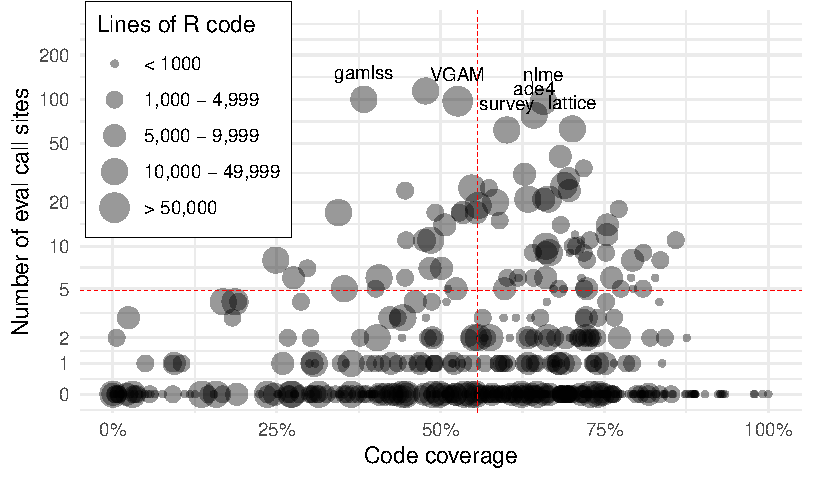
\includegraphics[width=.7\linewidth]
  {corpus.pdf}\caption{CRAN packages}\label{fig:corpus}
\end{figure}

To analyze a package, we need client code that invokes its methods.
There are three sources of built-in runnable code that come with each
CRAN package: \emph{tests, examples} and \emph{vignettes}. They are,
respectively, traditional unit tests, code snippets from the
documentation, and long-form use-cases written in Rmarkdown. Examples
and vignettes are automatically extracted and turned into scripts,
their input is bundled with the package. Most tests had to be discared
due to a limitation of our pipeline: the \c{testthat} harness uses
\eval and thus causes the entire test to register as an \eval call.
The selected packages are bundled with \CorpusPackagePrograms
programs; \CorpusExamplesProgramsRnd examples and
\CorpusVignettesProgramsRnd vignettes.

\mypara{Kaggle Scripts.} Kaggle is an online platform
for data-science and machine-learning. The website allows people to
submit data-analysis problems, users compete to find the best
solution. The solutions are uploaded to the platform as either plain
scripts or notebooks. We chose one of the most popular competition,
predicting the survival of passengers the
Titanic\footnote{\url{https://www.kaggle.com/c/titanic}}. Unlike CRAN,
Kaggle is not curated. After downloading the \CorpusKaggle solutions
and extracting the R code, we found that \CorpusDuplicatedKaggle were
duplicates. From the remaining \CorpusRunnableKaggle solutions,
\CorpusFailedKaggle failed to execute. Next to various runtime
exceptions, common problems were parse errors and misspelled package
names. The final set contains \CorpusFinishedKaggle programs
implemented in \CorpusFinishedKaggleCodeRnd lines of R code.



\subsection{Analysis Pipeline}

The results presented in this paper are the result of an automated
analysis pipeline that acquires the code of packages, extract
metadata, executes programs, traces their behavior and summarizes the
observations. Figure~\ref{fig:pipeline} shows the main steps of the
pipeline along with approximate time to execute each step, the data
size, and the number of elements manipulated by the stage. Timings are
for runs on an Intel Xeon 6140, 2.30GHz with 72 cores and 256GB of
RAM.

\begin{figure}[!h]\hspace{-5mm}
  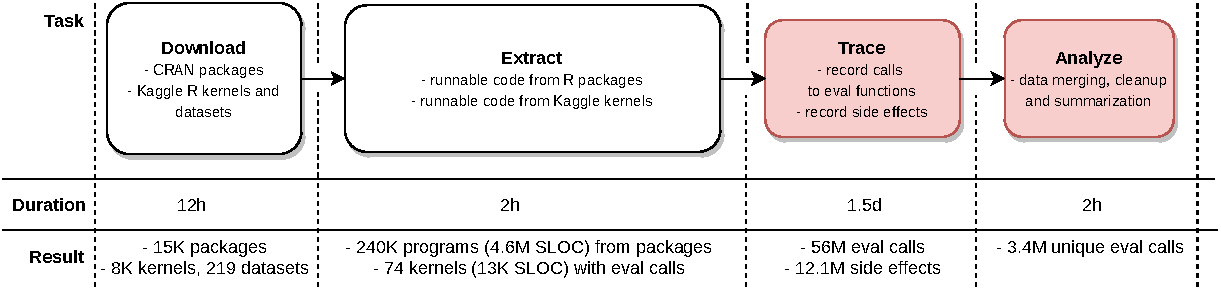
\includegraphics[width=1.05\linewidth]{pipeline.pdf}
  \caption{Analysis Pipeline}\label{fig:pipeline}
\end{figure}

The first step in the pipeline consist of downloading CRAN packages
along with their dependencies and acquiring Kaggle programs with the
help of a web crawler. The second step, is to compute code size and
coverage metrics for the CRAN packages (we use the \covr package for
coverage). The third step consist in extracting runnable programs from
packages: i.e. the tests, examples and vignettes. Each extracted
program is wrapped into a call to our dynamic analyzer --- the tool is
called \emph{evil} for \underline{ev}al \underline{i}nspection
\underline{l}ibrary. This step is needed to ensure that we record
\eval usage only for the target package. Without this, the data would
include eval calls from the unit testing frameworks as well as from
bootstrapping R virtual machine itself. To avoid any interference,
each program is run in its own R instance.
The fourth step in the pipeline is to perform dynamic analysis for
each run of a CRAN package or Kaggle program.

The dynamic analyzer builds upon the dynamic analysis framework,
\instrumentr that we have implemented to enable us to write dynamic
analysis logic in R. \instrumentr serves as an intermediary between
\rdyntrace and \evil, it intercepts the hooks exposed by \rdyntrace
and attaches R functions exported by \evil as callbacks. The \evil
callbacks execute on corresponding interpreter events.


The data extracted by \evil from each program is
concatenated, cleaned and summarized in the post-processing phase by
custom R scripts. Finally, the summarized data is analyzed in
RMarkdown notebooks to gather insights. Apart from the figures, the
data points included in the paper are also generated by RMarkdown
notebooks as latex macros.


The \emph{evil} framework is implemented as a R package in 2K lines of
R and 400 lines of C++ code. \instrumentr is an R package implemented
in 2.5K lines of R and 6K lines of C++ code. It internally uses a
modified R interpreter, \rdyntrace~\cite{oopsla19a}, that exposes
hooks from within the interpreter implementation for events of
interest.

All steps of this pipeline are parallelized using GNU
parallel~\cite{GNUparallel} and orchestrated by GNU make. To schedule
and parallelize extraction and analysis of programs, we use the \runr
package. Furthermore, \runr gracefully handles and reports failures
across large-scale program runs which greatly aids debugging of the
analysis pipeline.



\mypara{Limitations.} Dynamic analysis can only observe
calls that are triggered by the program's input. We believe that
focusing on R packages with high code coverage does mitigate this to
some extent. The results we report here were obtained with R's
bytecode compiler turned off, this should not affect the results as
the compiler does not optimize \eval.


. We turn off the
bytecode compiler for this study. The bytecode compiler can also call
\eval. We do not get source locations for \UndefinedEvalsRnd \eval
calls. In these cases \eval is either passed as an argument to a
higher-order functions or is defined in a function returned by a
higher-order function and the R parser does not retain location
information for \eval. However, this is a meager \PercentUndefinedEval
of all \eval calls and is unlikely to affect our analysis. We ignore
calls to the native \eval function exposed by R. We also ignore the
\c{rlang::tidy_eval} function which uses native \eval internally
because \c{rlang} is used to implement a DSL for data analysis in R.
It introduces a new first-class promise object called \c{quosure} for
which it implements special evaluation support in \c{tidy_eval}.


%%%%%
\section{Usage Metrics}

To provide a picture of \eval usage in R, we recorded \Allcalls
invocations of \eval and its variants in the CRAN corpus. These calls
were obtained by \Nbruns runs, with runs that did not trigger \eval
discarded. Out of the \NbStaticAtLeastOneCallSite CRAN packages(among the \Corpus packages of our corpus) with \eval call sites, we
observed calls in \Triggeredpkgs packages, the difference can be chalk
down to incomplete code coverage and occasional failures due to our
pipeline.

\begin{wrapfigure}{r}{5.2cm}
\begin{tabular}{|r@{\,}r@{\,}lr|r@{\,}r@{\,}lr|} \hline
\tt 0 &--& \tt 10      & \Bina  & \tt 1K &--&\tt 100K  & \Bine\\
\tt 11 &--& \tt 100    & \Binb  & \tt 100K &--&\tt 1M  & \Binf\\
\tt 101 &--& \tt 1K    & \Binc  & \tt 1M &--&\tt 10M   & \Bing\\
\tt 1K &--& \tt 10K    & \Bind  & \tt 10M &--& \tt 100M & \Binh\\\hline
\end{tabular}
\caption{Call frequency}\label{freq}
\end{wrapfigure}

Figure~\ref{freq} shows the number of \evals generated by each package
over all runs that invoked functions in that package. Out of the
\Corpus packages in the corpus, \Fewcalls packages have a low
frequency of \eval calls, with fewer than 100 of them. On the other
hand, \Manycalls packages call eval more than 1,000 times, with one
package (\Maxcallspack) calling it \Maxcalls times.

\begin{table}[h]
    \begin{tabular}{|c|c|c|c|c|}
        \hline
                       &\eval & \texttt{evalq} & \texttt{eval.parent} & \texttt{local} \\
        Dynamic & \Evals & \Evalqs & \Eparents & \Locals \\
        Static      & \Staticeval & \Staticevalq & \Staticevalparent & \Staticlocal \\
        Triggered & \Triggeredeval & \Triggeredevalq & \Triggeredevalparent & \Triggeredlocal \\
        \% triggered & \Triggeredevalpercent & \Triggeredevalqpercent & \Triggeredevalparentpercent & \Triggeredlocalpercent \\
        \hline
    \end{tabular}
    \caption{Variants of \eval}
\end{table}

\end{document}

(\EvalsRnd for \eval, \EvalqsRnd for \c{evalq}, \EparentsRnd for
\c{eval.parent} and \LocalsRnd for \c{local}).

\NbPackageEvalAtLeastOnce packages in our corpus call \eval at least once.

\mypara{Number of eval call sites.}  We observed that the number of
\eval call sites is small.  Figure~\ref{fig:callSitesPerPackage} shows
a violin plot of the distribution of call sites to \eval and its three
variants. For packages that have call sites, the median is
\NbMedianCallSites call sites. \NbOneCallSite{} packages have a single
call site, and one package, \emph{\MaxCallSitesPackage}, has
\MaxCallSites{} call sites. \PackagesNoCallsToEval{} packages have no
calls sites to \eval. These numbers are under-approximations as \eval
may be aliased, called reflectively and given as argument to a
higher-order function such as \c{map}.

\begin{figure}[h]
	\centering
	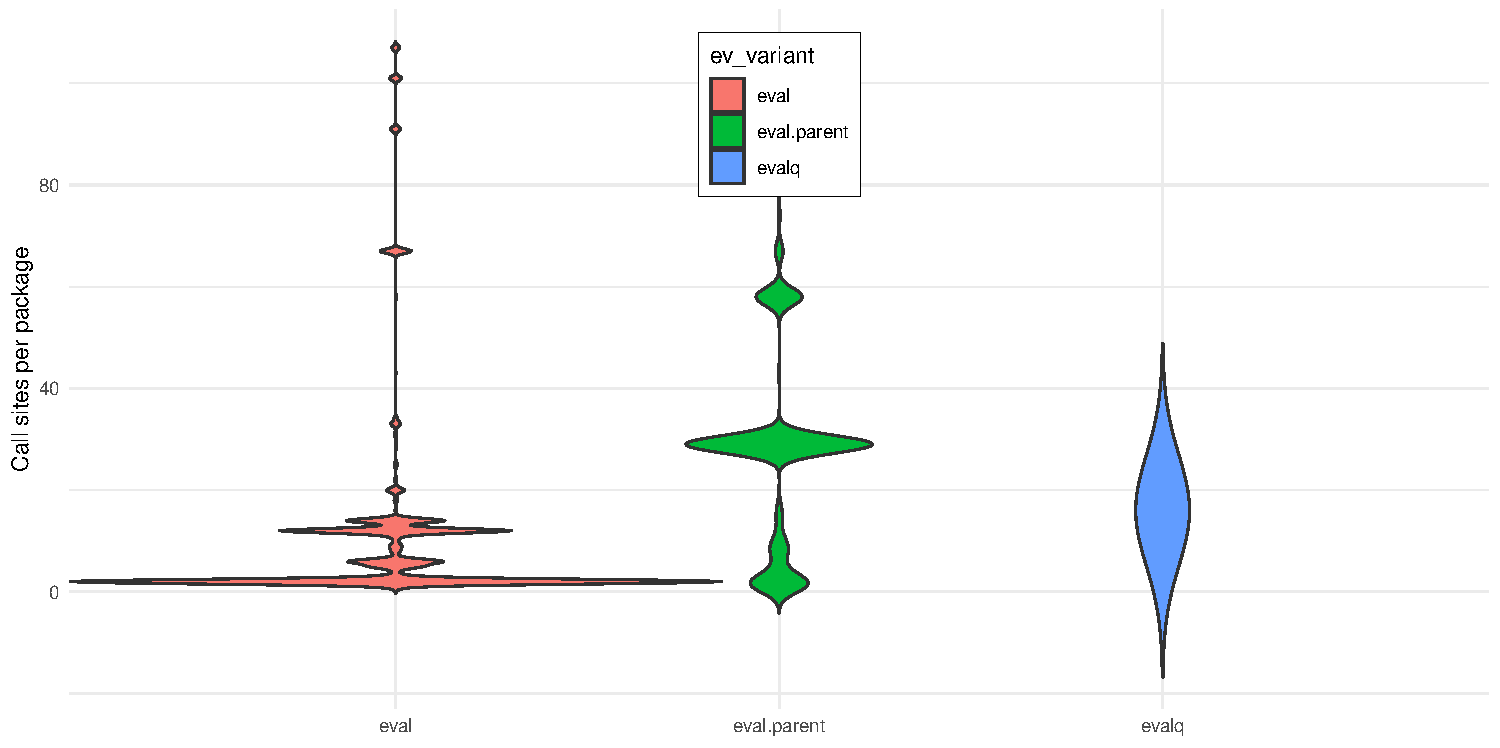
\includegraphics[width=\textwidth]{call_sites_per_packages}
	\caption{Violin plot of the call sites per packages per eval function. } \label{fig:callSitesPerPackage}
\end{figure}

\mypara{Number of calls to eval.} We observed an average \AverageEvalCallsPerPackage{} calls
to \eval per run. \NOTE{this is in packages that had any call to eval.
  How do we compute this? Say we are interested in package P. Do we
  only count runs that call eval from package P. Or do we also count
  runs that did not have an eval but executed some code from P? The
  latter may be easier. Which one is right?} Figure~\ref{fig:evalCallsPerPackage} shows a
violin plot of the distribution of calls to eval per run. The largest
number of calls per run is \MaxEvalCalls{} and comes from the package \MaxEvalCallPackage.

\begin{figure}[h]
	\centering
	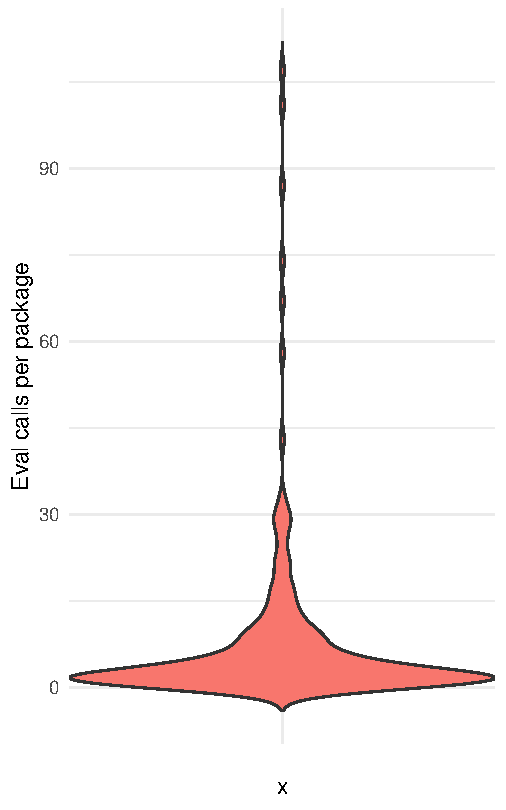
\includegraphics[width=\textwidth]{eval_calls_per_packages}
	\caption{Violin plot of the normalized number of eval calls per package. } \label{fig:evalCallsPerPackage}
\end{figure}

\mypara{Amount of code loaded by eval.} We use \c{deparse} to turn the
input to \eval into strings and measure the size of that input. The
largest input is \MaxSizeEval and the median input size is \MedianSizeEval. Most
inputs are small, less than \SizeNineFiveRnd bytes. The average size is \AverageSizeEval
bytes.

\mypara{Amount of computation via eval.}
We compare the number of events intercepted during execution of \eval
across the whole corpus. For this, we use the number of interpreter
steps as a proxy for events. We observe \AllEventCountRnd{} \NOTE{Check that number.\quad} events all
told, and \NbEventsEvalRnd events occur inside eval
(\EvalEventAllPerc of all events).
Figure~\ref{fig:eventsPerPackage} show a violin plot of events.

\begin{figure}[h]
	\centering
	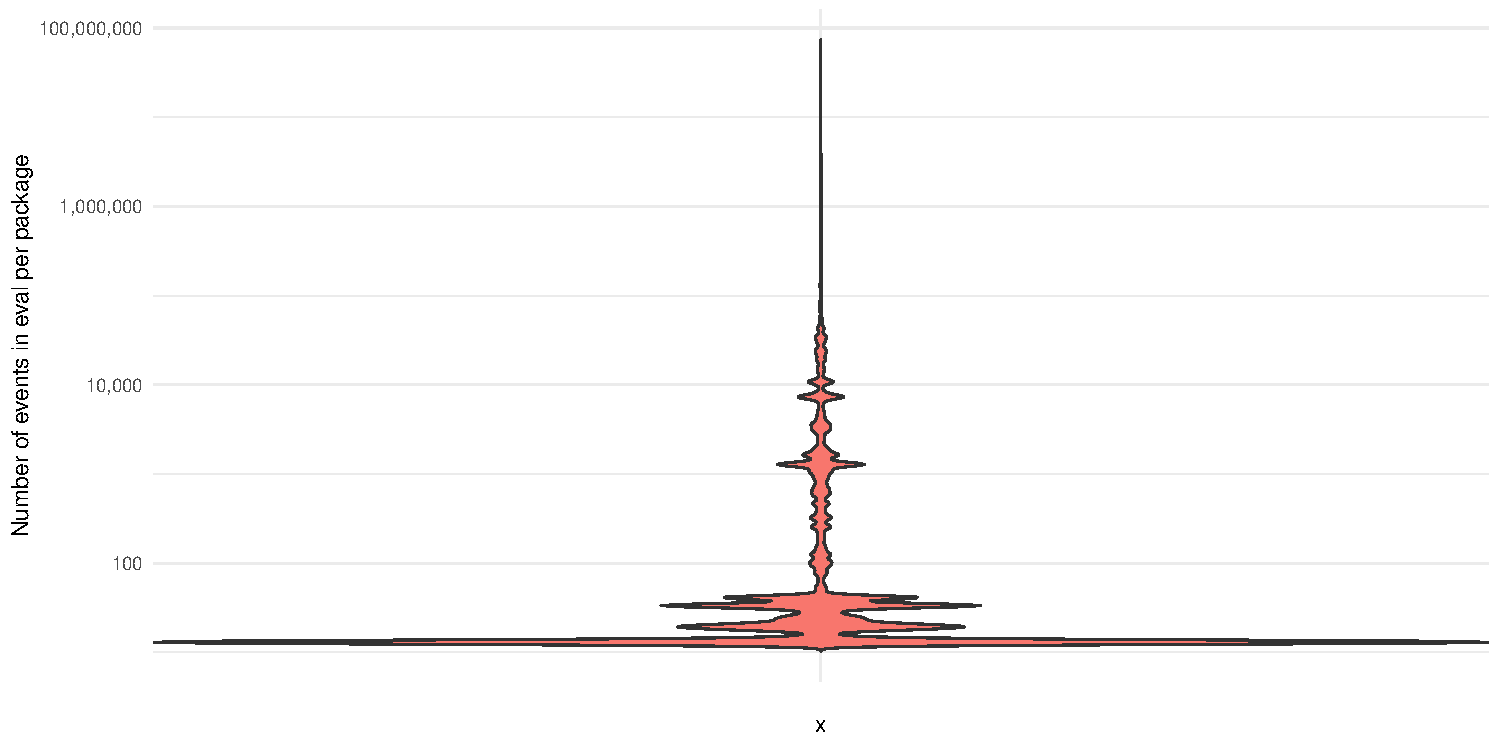
\includegraphics[width=\textwidth]{nb_events_per_packages}
	\caption{Violin plot of the number of events per packages (log scale). } \label{fig:eventsPerPackage}
\end{figure}

We observe a very wide spread in the number of events generated by
\eval calls. The largest number of events generated by an \eval call
is \MaxiEventsEvalRnd. However, a majority (\SmallEventsEval) of \eval calls performs up
to 100 events suggesting that most expressions passed to
\eval are small. It is interesting to note that a higher proportion of
Core R \eval calls perform side effects in the
\EventsMinRangeB--\EventsMaxRangeB range. Only \EventsCoreEvalCountC
Core R \eval calls and \EventsPackageEvalCountC package \eval call
generate \EventsMinRangeC to \EventsMaxRangeC events. These \eval
calls originate from statistical modeling packages such as \mlogit,
\mboost, \metafor, \lavaan, \mclust and \gamlss.

\NOTE{Talk about the percentage of code executed in eval}

\mypara{Eval Arguments.} Figure~\ref{fig:eval-expression-kind} breaks
down the expressions passed to \eval by R data type. It separates the
core packages from CRAN as they have different characteristics. In
core, XXX036\% of arguments in core are expressions. Whereas, in CRAN
package XXX037\% are expressions. When the argument is not an
expression, it is a value. Values are trivial for \eval as they are
returned unchanged. \PackageEnvironmentInputEvalCallPerc of CRAN
arguments are environments. This is an anomaly as only four \eval
call sites dominate this result:
\begin{compactitem}[$-$]
\item \c{ggplot2::ggproto} contributes to 99.9\% of package \eval
  calls that receive environments as input.
\item \c{R6::generator_funs} function contributes to only 936 \eval
  calls and implements the same functionality as \c{ggplot2::ggproto}
  but for the \emph{R6} OOP system.
\item \c{future::backtrace} function applies \eval to a future object
  which is implemented as an environment. This is called only once.
\item \c{RModel::str.RMmodel} function overloads the core \c{str}
  method for its \c{RModel} objects and maps \eval exactly like
  \c{str}. This is called only once.
\end{compactitem}



\begin{figure}[!h]
  \centering
  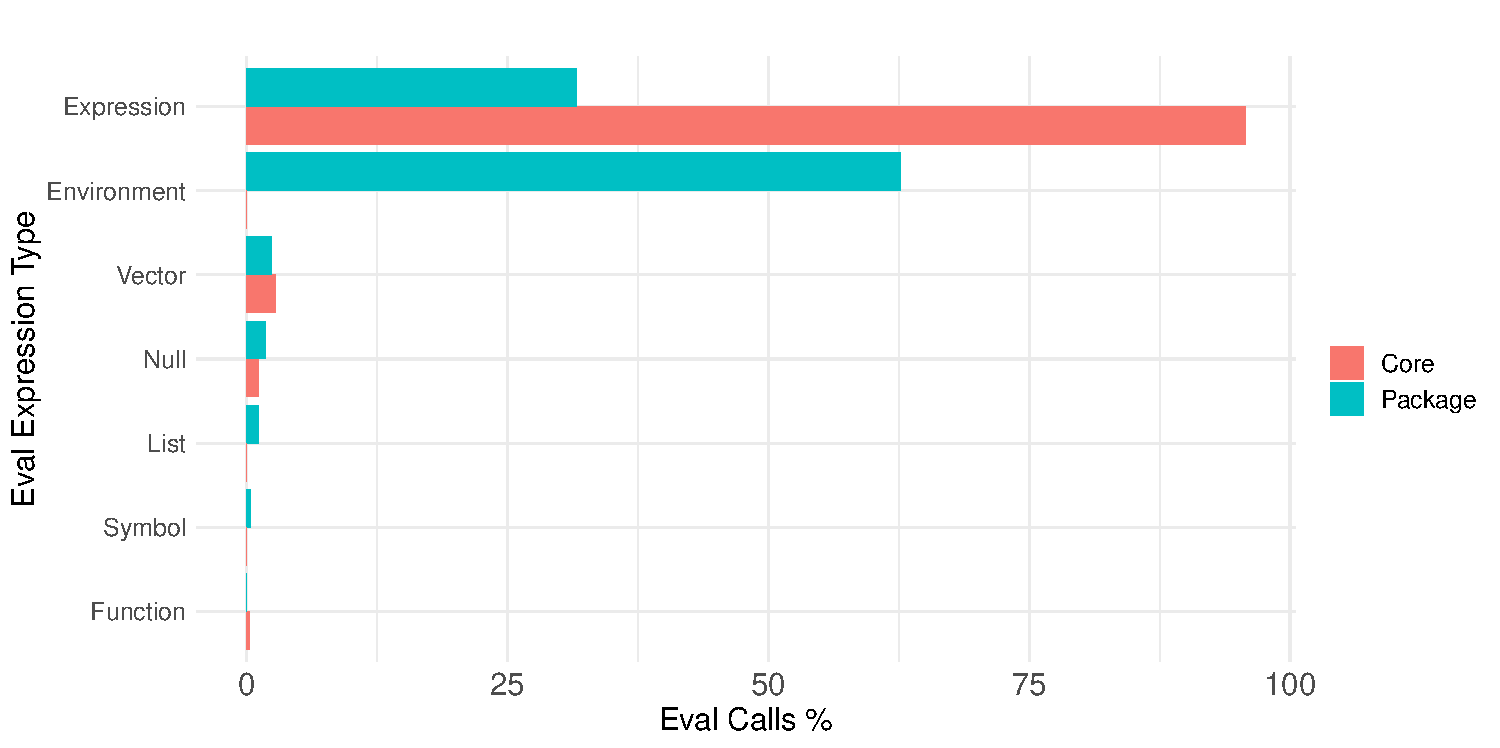
\includegraphics[width=\columnwidth]{eval-expression-kind}
  \caption{Type of Expression passed to \eval} \label{fig:eval-expression-kind}
\end{figure}




\mypara{The case of CORE libraries} ... \NOTE{Give numbers for the
  same things as above but for the base/core libraries} Compare.
\NOTE{Add XXX016 to XXX025.}



\section{A Taxonomy of Eval}

The previous section gave a quantitative view of the usage of \eval;
in this section we try to elucidate \emph{what} it does.

\mypara{Side-effects.} XXX026 total number of reads performed by
\eval. \NOTE{What is the definition of a read? An env lookup?} XXX027
average number of reads. XXX028 total number of writes performed by
\eval. Average number XXX029.

\NOTE{Aviral wrote''measure number of reads and writes by eval outside
  of its bubble'' --- what is the bubble here?}

XXX029 reads to caller environment -- where caller is the caller of
\eval.

XXX030 reads to other caller environment -- i.e. envs that are on the
call stack.

XXX031 reads to caller environment -- where caller is the caller of
\eval.

XXX032 reads to other caller environment -- i.e. envs that are on the
call stack.

Categorize side-effects between env passed to eval and other envs:
\begin{itemize}
\item ephemeral -- read to envs that are created during \eval  XXX033
\item local -- reads to env of the function in which the call to \eval
  lexically occurred; XXX034
\item parent -- reads to parent envs of the local one. XXX035
\item call-stack -- reads to envs that are on the call stack but not
  caller. XXX035.
\end{itemize}

In the corpus we observe \AllWritesRnd writes to variables of which
\EvalWritesRnd writes happen inside \eval. However, all writes are not
dangerous. Only writes to environments not local to the computation
spawned by \eval are side-effecting. These writes outlive the
computation and hence are visible outside it. The remaining writes are
local to the computation. We observe that \EvalSideEffectingWritesRnd
writes inside evals are side-effecting. This is only
\EvalSideEffectingWritesEvalPerc of all variable writes inside \eval
and \EvalSideEffectingWritesAllPerc of all variable writes in the
corpus.

An \eval is considered side-effecting if it performs a side-effecting
write to a variable, directly or indirectly. Only
\SideEffectingCoreCallPerc \eval calls in Core R are side-effecting
and \SideEffectingPackageCallPerc \eval calls in CRAN packages are
side-effecting.


\mypara{New Bindings.} Find number of times, eval introduces new
bindings. There are many ways -- library, load, attach, source, and
explicitly introduce bindings using super-assign, assign and define.

\mypara{C Calls.} Find number of times, eval makes call to native code
using - .Call, .External, etc. Find out if there are native functions
that are called only from within eval.

\mypara{Non-local returns}
Eval can do non-local returns effective bypassing evaluation of the
rest of the function. This can be useful for static analyzers.

\mypara{Purity.}
Conclude with number of evals that are ``pure'', i.e. evals which
could be ignored by a static analyzer without any problem.

\mypara{Source.}
There are various ways to obtain expressions:
\begin{itemize}
  \item \c{substitute} synthesizes ASTs from expressions by replacing
    symbols with their bindings in the specified environment.
  \item \c{expression}  creates a vector of expression
    objects from text.
  \item \c{parse}, \c{str2expression} and \c{str2lang} turn strings into
    expressions.
\end{itemize}

We observe 5.2\% cases where \eval directly evaluates the output of
\c{substitute}, 0.7\% cases where output of \c{parse} is read directly
and only 704 cases for \c{expression}. Most expressions consumed by
\eval are generated by other functions.

\c{eval(parse(...))} can be used for dynamic code loading. This forms
the core of \c{source} and \c{sys.source} functions in R that are
commonly used for loading code in R files in interactive settings. We
investigated the number of cases in which the output of \c{parse} and
its variants is passed to \eval, directly or transitively by tainting
their output. This corresponds to \PercentParsedCallSites of the total
\eval call sites and \PercentParsedEvals of the eval calls. We
observed that very few of the eval call (\NbParseFilesRnd in total)
consume the result of calling \c{parse} on a file. Most of the eval
calls consume the result of calling \c{parse} on a string. We also
identified one function in core R, \c{invokeRestartInteractively} that
prompts the user for input, parses it, and passes it to \eval.


\mypara{Scope.} The environment argument can be \c{NULL}, a \c{List}
or a data frame. This happens in 3.5\% of the cases: \eval copies the
fields of the list or data frame and creates bindings for them in a
new environment. This pattern is used to evaluate formulas which can
directly refer to the fields of the data. The \c{envir} argument can
also be a number $n$. It means that the environment in which the
expressions is evaluated will be the result of \c{sys.call(n)} where
$n$ refers to the $n$-th stack frame.

The top-level environment in R is called the global environment. New
environments can be created using \c{new.env}. They can be provided a
parent environment which becomes the enclosing scope of the new
environment.

We looked at the environments passed to all the \eval calls in our
corpus. Table~\ref{tab:environments} summarizes the results. A numeric
environment class \c{n} denotes the environment of the $n$-th call
stack frame from the current function. \c{global} denotes the
top-level environment and \c{list} denotes a list passed for
evaluation of formulas. Environment classes of the form $n+$ denote
the $n$-th environment extended with a new environment. The new
environment provides a limited form of sandboxing. All assignments
using the \c{\<-} function occur inside it and prevent the extended
environment from mutation. However, it is still possible to mutate the
extended environment using the \c{\<\<-} or \c{assign} functions; but,
that happens rarely.

\begin{table}[htbp]{ \centering
\begin{tabular}{c|c|c|c}\hline
\multicolumn{2}{c|}{Core} & \multicolumn{2}{|c}{Packages}  \\\hline
Environment Class & Eval Calls \% & Environment Class & Eval Calls\\\hline
\CoreEnvClassA & \CoreProportionA & \PackagesEnvClassA &  \PackagesProportionA\\
\CoreEnvClassB & \CoreProportionB & \PackagesEnvClassB &  \PackagesProportionB\\
\CoreEnvClassC & \CoreProportionC & \PackagesEnvClassC &  \PackagesProportionC\\
\CoreEnvClassD & \CoreProportionD & \PackagesEnvClassD &  \PackagesProportionD\\
\CoreEnvClassE & \CoreProportionE & \PackagesEnvClassE &  \PackagesProportionE\\\hline
\end{tabular}} \label{tab:environments}
\caption{Environments in terms of \eval calls}
\end{table}

We observe that a disproportionately high number of core R \eval calls
access the caller's caller's environment. This is because many core R
functions call functions that pass the result of \c{parent.frame()} to
an \eval. A disproportionately high number of calls to \eval happens
in an extended top-level environment. This can be explained by the
fact that many packages evaluate code passed from the user's workspace
in the top-level environment to access the bindings.


The \c{imchange} function of package \c{imager} makes it possible to
modify images using a dedicated formula syntax using
\c{\~}.\footnote{Inspired by {map} in package \emph{purr}.} Here,
\eval is evaluated in \c{newenv}, which creates a new environment that
inherits from \c{parent.frame()} by default (classified as 1+).


\begin{lstlisting}
newenv <- new.env()
...
fo <- parse(text=as.character(fo)[2])
im[where] <- eval(fo,envir=newenv,enclos=env)
\end{lstlisting}

\c{adjCoef} in package \emph{actuar} find the root of an equation
defined by a function \c{h} whose arguments must be named \c{x} and
\c{y}. \c{h} is transformed into an auxiliary function \c{h2} that can
be optimized. Here, the list used for \c{envir} ensures the
correspondance between the textual arguments of \c{h} and the
arguments of \c{h2}.


\begin{lstlisting}
sh <- substitute(h)
fcall <- paste(sh, "(x, y)")
...
h2 <- function(x, y)
    eval(parse(text = fcall),
    envir = list(x = x, y = y),
    enclos = parent.frame(2))
\end{lstlisting}


\section{Case Studies}

\NOTE{5(?) examples from real code?}

\subsection{LEGACY TEXT}

We looked at the top ten expressions passed to core and package \eval
calls. The most frequent ten expressions to eval calls from core R
contribute to 85\% of all \eval calls.

\begin{table}[!h] \centering
\begin{tabular}{@{}l|rr@{}} \hline
Expression & Eval Call &  \% \\\hline
\c{c("auto", "shell", "radix")} & 1,987,105 & 29\%\\
\c{c("auto", "shell", "quick", "radix")} & 1,593,169  & 23\%\\
\c{\{info <- loadingNamespaceInfo(...} & 1,008,632 &       14\%\\
\c{c("onLoad", "attach", "detach", "onUnload")}   & 470,566 &      6.9\%\\
\c{c("append", "prepend", "replace")} &              261,587&       3.9\% \\
\c{c("left", "right", "centre", "none")} & 162,086     & 2.4\%\\
\c{c("no", "ifany", "always")}   &                71,580 &       1.1\%\\
\c{c("pearson", "kendall", "spearman")}  & 72,962 &      1.1\%\\
\c{NULL}& 75,330  &      1.1\% \\
\c{Symbol}&                 66,279&       1\%\\\hline
\end{tabular}
\caption{Top ten eval calls in Core}\label{B}
\end{table}

The expression \c{\{info <- loadingNamespaceInfo(...} is added by core
R to a package directory during installation. To load the package,
this code is executed. It creates a namespace for the package, injects
the package bindings, and attaches the namespace to the program search
path. The \c{NULL} comes from a call to \c{substitute(subset)} in
\c{stats::model.frame.default} function which has a default value of
\c{subset} as \c{NULL}. The \c{Symbol} arises from a call to
\c{as.name} in \c{base::str} function that returns a symbol that is
looked up by evaluating it in a specific environment. The remaining
cases arise from calls to \c{match.arg} which is used to look up the
default choices for a variable and match against the choice passed by
the caller.

The most frequent ten expressions to eval calls from CRAN packages
contribute to 77.1\% of all \eval calls.

\begin{table}[!h]  \centering
\begin{tabular}{@{}l@{~}|@{~}r@{~}r@{}} \hline
Expression & Eval Call &  \% \\\hline
\c{Environment} &                                  989302   & 61\%\\
\c{column[rows] <<- what} &                        55677    & 3.5\%\\
\c{function(value) freduce(value, `_function_list`)} & 37251& 2.3\%\\
\c{NULL} &                         32005    & 2\%\\
\c{List} &                         22293    & 1.4\%\\
\c{c("default", "default2012", "default2011" ...}& 20610    & 1.3\%\\
\c{force(..1)}            &                        20461    & 1.3\%\\
\c{alist(`_spec`)}       &                         18532    & 1.2\%\\
\c{inner}               &                          18530    & 1.2\%\\
\c{String Vector}      &                           17487     & 1.1\%\\
\end{tabular}\caption{Top ten eval calls in CRAN} \label{C}
\end{table}

The expression \c{Environment} occurs because of the four callsites
explained above, \c{ggplot2::ggproto}, \c{R6::generator_funs},
\c{future::backtrace} and \c{RModel::str.RMmodel}. The next
expression, \c{column[rows] <<- what}, is used inside the
\c{plyr::rbind.fill} function to merge data frames by assigning
concatenated vectors to rows. The \c{<<-} operator is interesting in
that it skips the current scope and assigns in a parent scope in which
the variable is already present. In our corpus, all these \eval calls
contribute to a single side-effect. The expression \c{function(value)
  freduce(value, `_function_list`)} arises from the
\c{magrittr::\%>\%} function which is a pipe operator that pipes the
output of previous command to the next one. The expression is
evaluated in a custom environment to create a function binding for
evaluating the components of the pipe.\c{String Vector} and \c{List}
also arise from the same function when a string or a list is piped
using the \c{\%>\%} function into the next expression. The \c{NULL}
arises from \c{R6::generator_funs} function when the \eval is passed a
\c{NULL} argument by the \c{DataMask_generator} package. The
\c{c("default", "default2012", "default2011" ...} pattern arises from
\c{copula::polyG} where it reflectively access the default expression
for its formal parameter and evaluates it. The \c{force(..1)} and
\c{alist(`_spec`)} patterns occur in \c{glue::glue_data} function
which concatenates and interpolates strings. The two patterns occur
because the function captures unevaluated unnamed arguments and maps
the evaluation of \c{force(..1)} on them. The \c{force} function
forces promises and returns the result of evaluation. The \c{inner}
pattern arises from \c{glue::identity_transformer} which enables the
creation of custom transformation functions for affecting the
interpolation and concatenation of input by the \c{glue} package.


\section{Why do we Eval}

\subsection{Discussion}

Yeah, why?

\subsection{Can we do without?}


We look at how \emph{consistent} the \c{expr} argument of \eval can
be, \ie how many different types of the resolved \c{expr} there are
per call sites. Most of the call sites, \ie \PercentMonomorphic, are
\emph{consistent}, and this is similar to javascript. However, a few
ones are highly \emph{polymorphic} (10 different types). They are the
pipe operators \c{\%>\%}, \c{\%<>\%} and \c{\%\$\%} in package
\emph{magrittr}. It is effectively used to compose functions on their
first argument, which can be of any type.

Similarly to JavaScript, there are also unnecessary uses of \eval. For
example, the \c{PerformanceAnalytics} package contains a function
\c{chart.QQPlot} that uses \eval to resolve a string into function and
another to call it and assign its results into a variable:
\begin{lstlisting}
function (R, d="norm", dp, ...) {
q.f <- eval(parse(text=paste("q",d,sep="")))
z <- NULL
eval(parse(text=paste("z<-q.f(",dp,",...)")))
}
\end{lstlisting}
  In both cases, there is no need for \eval:
\begin{lstlisting}
function (R, d="norm", dp, ...) {
q.f <- get(paste0("q",d))
z <- q.f(dp, ...)
}
\end{lstlisting}
  or even to a oneliner \c{do.call(paste0("q",d), as.list(dp, ...))}.

\subsection{Comparison with Javascript}



\section{Conclusion}



\bibliography{bib/bibliography,bib/jv}

\end{document}
